%definición del artículo
\documentclass[a4paper,12pt,openany,oneside]{book}
\usepackage[left=5cm,right=2cm,top=4cm,bottom=4cm,paperwidth=216mm,paperheight=330mm,pdftex]{geometry}
%paquete usado para silabación en español
\usepackage[spanish]{babel}
%codificación del documento
\usepackage[utf8]{inputenc}
%espaciado
\linespread{1.5}
%identación de párrafo
\setlength{\parindent}{20pt}
%espaciado de párrafo
\setlength{\parskip}{4ex plus 0.5ex minus 0.2ex}
%para validar sólo sintaxis sin compilar
%\usepackage{syntonly}
%\syntaxonly
%para usar imágenes
\usepackage{graphicx}
%para usar fragmentos de codigo fuente
\usepackage{listings}
\usepackage{float}
%para usar signos de check y wrong
\usepackage{bbding}
%para usar colores en textos y simbolos
\usepackage{color}
\usepackage{multirow} %multi columna
\floatstyle{boxed}
\newfloat{codigo}{thp}{lop}
\floatname{codigo}{Caja de Código}

%comienzo del documento
\begin{document}
%\thispagestyle{empty}

\begin{center}

\pagenumbering{gobble}
\textbf{UNIVERSIDAD TECNOLÓGICA METROPOLITANA\\
FACULTAD DE INGENIERÍA\\
ESCUELA DE INFORMÁTICA}\\
\vspace{3cm}
\textbf{MÓDULOS INTEGRADOR Y MANTENEDOR DE DATOS EN SISTEMA SEPA}
\end{center}
\begin{flushright}
\textbf{TRABAJO DE TÍTULO PARA OPTAR AL TÍTULO DE\\
INGENIERO CIVIL EN COMPUTACIÓN MENCIÓN INFORMÁTICA\\}
\vspace{3cm}
\textbf{PROFESOR: Sebastián Salazar Molina\\}
\vspace{1.5cm}
\textbf{ALUMNO: Miguel Ángel Aníbal Davor Fuenzalida Pino}
\end{flushright}
\vspace{4cm}
\begin{center}
\textbf{SANTIAGO - 2015}
\end{center}
\newpage
\thispagestyle{empty}
\begin{flushright}
\vspace{20mm}
Nota: \line(1, 0){140} \\
\vspace{30 mm}
\line(1, 0){180}\\	
Firma y Timbre\\
Autoridad Responsable
\end{flushright}
\chapter*{Resumen}
\thispagestyle{empty}
% En las organizaciones es necesario el uso de información para tomar decisiones correctas.
% Tener un buen software, entrega valor agregado a la dirección de actividades en todo tipo de estructuras con jerarquía.

La UTEM dispone del sistema SEPA (Sistema Estadístico de Profesores y Alumnos), que consiste en un proyecto Web realizado con anterioridad, que toma datos de alumnos, profesores y encargados provenientes de DirDoc, para posteriormente obtener indicadores que representen la realidad universitaria.

Sin embargo SEPA presenta insuficiencias, por ejemplo: no dispone de un mecanismo que se comunique con DirDoc de manera segura y controlada, tampoco presenta formas alternativas de acceso, no posee varios tipos de roles y tiene datos incompletos.

% ejemplos, no tiene servicio web dirdoc, inconsistencia de datos, carece de formas alternativas de accesos, carece multiples roles (más de 2).

El presente trabajo de título ofrece una actualización al sistema SEPA, con integración de herramientas que permiten mejoras por la Universidad, explicadas a fondo en este informe.

El resultado final de este proyecto es la obtención por parte de la Universidad de un servicio que comunique SEPA con DirDoc de manera más expedita y segura, mediante varios tipos de consultas con un módulo de mantenedor que permitirá monitorizar y editar las distintas tablas mediante sus registros correspondientes, pensado desde un principio para hacer búsquedas y reparar data que este incompleta.

\chapter*{Summary}
\thispagestyle{empty}

The UTEM has the SEPA system (Statistical System of Professors and Students), which consists of a Web project done before, which takes data from students, teachers and managers from DirDoc, later to obtain indicators that represent the university reality.

However SEPA has shortcomings, for example, it doesn't have a mechanism to contact DirDoc safe and controlled way, nor has alternative access ways, it doesn't have many types of roles and it has incomplete data.

This work provides an update to the SEPA system, with integrated tools that allow improvements by the University, explained in depth in this report.

The final result of this project is to obtain by the University to provide a service that connect DirDoc with SEPA more expeditiously and safely, using various types of consultations with maintainer module allowing you to monitor and to edit the different tables using corresponding records, designed from the start to search and repair data that is incomplete.

\tableofcontents
\listoffigures
\listoftables
\thispagestyle{empty}
\chapter*{Introducción}
La Universidad Tecnológica Metropolitana (UTEM) utiliza para la administración de toda la información referente a estudiantes, profesores y personal de administración un sistema denominado DirDoc (ver anexo), basado en la tecnológica PHP (ver anexo). SEPA, software desarrollado por Sebastián Salazar Molina, mediante el lenguaje de programación PHP, como trabajo de título, siendo proyecto que constituyó una forma de potenciar las capacidades operativas de la Universidad, generando indicadores de calidad y entregando una ventaja comparativa frente a otras Universidades.

El objetivo de este trabajo de título consiste en mejorar el proyecto SEPA mediante la programación en Java que utiliza herramientas estructuradas, extensibles y que tienen como resultado la materialización de sistemas informáticos de más fácil mantención debido al uso de Patrones de Diseño como Modelo Vista Controlador sobre tecnologías como Java EE, JPA, Spring, JSF, PrimeFaces, ver anexo.

Además, el proyecto se planificará mediante el uso de la metodología PSP (Personal Software Process) que nos proporciona un modelo de trabajo basado en la caracterización de los tiempos y costes de operación de un ingeniero informático, adicionando documentación extra (explicada en este informe), correspondiente a eventos que muestran cómo se lleva adelante esta tarea, todo lo cual, conduce a una evaluación de la calidad del proyecto como programa.

Existen 3 tipos de beneficios que la Universidad puede obtener al utilizar con la versión mejorada del sistema SEPA:

\begin{enumerate}
\item Una panorámica de la realidad universitaria, para tener una visión general de la realidad universitaria, sin olvidar la perspectiva particular de cada fortaleza y debilidad. Permitiendo una rápida detección de los problemas que puedan surgir. Generando una posibilidad de mejoras en los funcionamientos internos y externos de la organización.

\item Beneficio de los usuarios que tendrán a su disposición una completa herramienta que los apoyará en la elección de su carga académica, como asimismo la visualización de su desempeño.

\item Beneficio a futuro, dado el gran tiempo de utilidad de las herramientas que permiten automatizar la integración de la data resultando más sencilla.
\end{enumerate}

La justificación principal de por que en SEPA se realizarán estas mejoras, radica en la necesidad de contar con indicadores actualizados y precisos, que son los que hacen que las decisiones sean justificadas. Por ejemplo, una vez implementadas las mejoras, en SEPA se prodrá fácilmente programar contadores de la totalidad de las tablas, incluidas conexiones entre tablas, mientras que la version actual de SEPA tiene contadores simples y poco específicos, tales como el promedio de notas por ramo y por alumnos programados, de manera tal que no se pueden hacer búsquedas específicas sobre todos los parámetros de una tabla.

Otra justificación de estos cambios, es la capacidad de reparar datos que esté mal escrita o que simplemente no exista, permitiendo que los datos puedan ser mejorados constantemente y de manera automática. Característica que SEPA actual no posee, ya que para solicitar un cambio se necesita básicamente pedir los datos desde la propia fuente, proceso que es manual, toma días y requiere de muchas personas. 

Finalmente es importante destacar que las transacciones de los servicios web que se agregaran como parte de este proyecto constituyen otra mejora, haciendo el sistema más seguro y rápido.

\chapter{Antecedentes}
\pagenumbering{arabic}
\thispagestyle{empty}
\section{Contexto General}
La Universidad Tecnológica Metropolitana (UTEM) es un organismo de enseñanza superior que se encuentra dentro del Consejo de Rectores de las Universidades Chilenas. Dentro de su sistema administrativo de notas se ocupa el sistema DirDoc, el cual entrega información de notas con respecto alumnos y asignaturas y es ocupado particularmente por alumnos, profesores y directores de escuela para  mirar e ingresar notas, de los distintos ramos impartidos en la Universidad. SEPA es una herramienta que nació como un apoyo en el ámbito estadístico para tomar los datos que se encuentran en el marco de DirDoc, permitiendo obtener valores ponderados entre otras cosas.
\section{Contexto Particular}
El proyecto SEPA, Sistema Estadístico de Profesores y Alumnos, es el encargado de mostrar información que puede ser cuantificable en pos de tener herramientas de control general y toma de decisiones. Dicha información viene del sistema DirDoc que se utiliza para la mantención de datos académicos en la Universidad.

\section{Motivación}
Ayudar a mejorar las herramientas de administración de la Universidad y aprender a desarrollar tecnologías que apoyen a las instituciones de educación.
Para lograr esto se llevarán a cabo las siguientes tareas:
\begin{itemize}
	\item Acceder a un servicio web para obtener los datos de manera segura. Esto implica la creación de componentes que consuman los servicios del Dirdoc. Estos a su vez son un conjunto de procesos que cargan información en una base de datos, teniendo especial cuidado en datos que estén corruptos o con falta de información. Intentando guardar en la medida de lo posible, toda la información necesaria.
	\item Crear un mantenedor de todos los datos que podamos integrar en el servicio web. Este mantenedor tendrá como objetivo ser una herramienta de múltiples propósitos, tales como visualizar o reparar data. Tener permisos que restringan el acceso a los usuarios del sistema.
	\item Automatizar los procesos de acceso y actualización de datos mediante ejecuciones que se efectúen de manera automática. Estos procesos deben hacer uso de los servicios web en horarios específicos, destinados a ocupar el procesamiento del servidor en horas en que no hay mucho flujo de data.
\end{itemize}

\chapter{Problema}
\thispagestyle{empty}
\section{Situación Actual}
\subsection{Dirdoc}
El Dirdoc es una plataforma online a la que alumnos, profesores y funcionarios tienen acceso, mediante distintos medios, En cada uno de estos se ejecutan ciertas actividades. A continuación se detallan sus características.

\begin{itemize}
	\item Estudiante: Es un acceso que le permite a un alumno mirar sus notas y sus promedios de todos sus ramos, además de la carrera, la maya curricular, entre otros.
	\item Profesor: Es un acceso en el que se permite la inserción de notas para los alumnos correspondientes, de acuerdo a los ramos que se imparten. Entre otras cosas, es posible buscar información del profesor, ramos en los que trabaja y alumnos asociados a las clases.
	\item Gestor: Son capaces de buscar información de todos los otros niveles, e incluso tienen facultades para editar información, para lo cual su uso esta centrado en regular el correcto funcionamiento de la herramienta DirDoc y tomar acciones frente a errores que puedan originarse.
\end{itemize}

\subsection{SEPA}
El SEPA (Sistema Estadístico de Profesores y Alumnos) es una herramienta complementaria en la UTEM que otorga principalmente indicadores estadísticos, que permiten tomar decisiones que afectan a un segmento importante de la organización. Por ejemplo se tiene el promedio de notas de un curso que imparte un profesor, o también el promedio de notas totales de un alumno. Si bien son importantes estos datos, son poco específicos.

Uno de los problemas que se tienen en sepa, es que al no existir un sistema de ingreso de data desde DirDoc, la única forma de ingresar data en sepa es mediante la petición a un funcionario encargado del sistema, lo que supone un riesgo por la perdida de data. Las principales insuficiencias en SEPA son:

\begin{itemize}
	\item No se dispone de un mecanismo para actualizar datos (una forma de acceso más segura y controlada) de DirDoc. En el actual SEPA se deben seguir una serie de pasos para ingresar data. Primero se debe seleccionar mediante el DirDoc que data hay que insertar en SEPA y después se requiere hablar con un encargado de SEPA para que ejecute una sentencia SQL que ingrese los valores deseados a la base de datos. Lo que conlleva peligro, ya que es muy probable la perdida u omisión de algún valor.
	\item Falta de datos. Retomando el punto anterior, en el actual SEPA presenta tablas que no tienen datos y esto es debido a que en su proceso de inserción, estos fueron omitidos o perdidos.
	\item No posee acceso de múltiples tipos de usuarios, diferenciados por actividad. Lo que constituye una barrera ya que actualmente no se puede mostrar toda la información para la cual un rol tiene acceso, por ejemplo, un profesor debiera ver su información y la de sus alumnos, pero un jefe de carrera debe ser capaz de ver su información, la de los alumnos y la de los profesores. 
	\item No existe una forma sencilla de modificar y actualizar la información desde DirDoc hasta SEPA, ya que lo que hoy se esta haciendo es hacer una petición sobre una data en DirDoc y finalmente pedirle a un encargado que ingrese cierta data a la base de datos de SEPA
\end{itemize} 


\section{Situación Propuesta}
Dentro de los módulos mantenedor e integrador de SEPA se comprenden las siguientes actividades que no están en la versión anterior:

\begin{itemize}
	\item Ingreso por perfiles: Gracias a las mejoras que se programan, se agrega el sistema de registro por perfiles, el cual otorga permisos por los distintos tipos de usuarios. Estos tendrán un rango de data que puedan visualizar. 
	\item Visualización de todas las tablas: En estas mejoras a SEPA se incorpora la posibilidad de mirar todos los parámetros de las tablas comprendidas en el modelo de base de datos. Esto significa que mediante los perfiles es posible ver la información historia de todas las tablas permitidas.
	\item Edición de todas las tablas: Como en el punto anterior, no solo es posible mirar, ya que también hay perfiles que pueden editar data de las tablas, pensando en la reparación de esta debido a que puede tener fallos o faltar.
	\item Integración por web service: El traspaso de data desde DirDoc a SEPA será mediante un servicio en linea de comunicación entre dos programas (DirDoc y SEPA), ya que de esta forma uno se asegura que la forma de ingreso de data en SEPA sea, en la mayor medida, limpia y sin errores. El sistema es capas de soportar la falta de ciertos datos en las tablas, los cuales pueden ser llenados posteriormente por el mantenedor que se incorpora.
	\item Facilidad de programar indicadores en un futuro: La forma de como esta programado SEPA supone una mejora, ya que al utilizar una tecnología que al ser de un código maduro, posee una fácil mantención, es simple encontrar otros desarrolladores que aporten con la programación de distintos indicadores. Ya que solo basta que se tenga gente con conocimientos específicos del entorno del servicio y la vista, sin conocer en detalle el modelo de la aplicación.
\end{itemize}
\section{Objetivos Generales y Específicos}
\subsection{Objetivos Generales}
\textit{Mejorar SEPA convirtiéndolo en un sistema actualizado e independiente de información estadística para la Universidad Tecnológica Metropolitana ayudando a sus procesos docentes y productivos, disponiendo de información veraz de la realidad universitaria.}

A partir de la versión actual de SEPA, crear un sistema web basado en el patrón Modelo Vista Controlador, asegurando un producto que sea eficiente en el cumplimiento de sus objetivos. Las características principales serán que este sistema estará hecho en Java lo que nos permite una fácil implementación de las mejores prácticas de programación. Potenciando su valor en el tiempo, convirtiéndose en una herramienta cada vez mas útil y necesaria para el desarrollo de la organización.

\subsection{Objetivos Específicos}
\begin{enumerate}
	\item Generar un sistema que sea fácilmente mejorable, usando tecnologías estandarizadas y óptimas. Mediante JavaEE (Java Enterprise Edition), lo cual permite la integración de herramientas robustas dentro del software, tales como un sistema de mapeo de bases de datos a objetos simples de ocupar, un servicio web de comunicación entre dos sistemas, una vista con elementos de fácil interacción con el usuario final, entre otros.
	\item Entregar un producto de calidad, escalable y fiable para la comunidad universitaria. El cual sea un aporte para la toma de decisiones y también un soporte en la búsqueda de patrones o mejoras administrativas.
	\item Utilizar una metodología de desarrollo, en este caso PSP (Personal Software Process), la cual nos permite llevar un seguimiento y retroalimentación de las actividades que se deben realizar, de manera lógica y ordenada. Para este propósito la metodología propone la utilización de valores contables en el tiempo, estos valores establecen las características y condiciones del trabajo del ingeniero. Lo cual entrega valor agregado al producto, mostrando data numérica y estadística del tiempo invertido en el trabajo y como este se va completando con eficiencia.
	\item Hacer una mejora sustancial en SEPA de manera que todo su conjunto sea útil para todos los usuarios a los que se enfoca, haciendo especial énfasis en que los perfiles a los que esta dirigido este trabajo puedan certificar mejoras en la calidad de la data, la rapidez del servicio, la seguridad ofrecida.  
	\item Producir una herramienta moderna, que cumpla con calidad el objetivo propuesto, siendo un desafío para el desarrollador, incorporar herramientas simples que entreguen producto robusto y confiable, sin comprometer la factibilidad de desarrollo futuro.
\end{enumerate}
%\chapter{Alcances y Limitaciones}
%\thispagestyle{empty}
%\section{Alcances del Proyecto}
%La coparticipación de indicadores UTIGRA (Unidad de títulos y Grados) para trabajar con información pertinente a %gente que ha terminado sus procesos estudiantiles en la UTEM.

%Se crearan una serie de nuevos perfiles, y cada uno de estos tendrán su nivel de alcance en el sistema.
%\section{Limitaciones del Proyecto}
%El proyecto no contendrá requerimientos que se hagan fuera de lo requerido por el profesor como actividades de %Trabajo de título.
%\section{Alcances del Trabajo de título}
%Los alcances del Trabajo de título están delimitados por las características que el trabajo de título debe tener, es %decir, que se hace un marco de trabajo, delimitado por el profesor, que comprende los tópicos a trabajar.
%\section{Limitaciones del Trabajo de título}
%El trabajo no comprende áreas que estén fuera de los límites temporales a la toma de requerimientos, por lo cual es %necesario indicar que hay características y funcionalidades que a pesar de ser levantadas puede que no sean parte de %este trabajo de título.
\section{Estructura de desarrollo el proyecto}
El desarrollo del proyecto se realiza bajo la metodología Personal Sofware Process (PSP), la cual permite medir en forma cuantitativa todas la variables implicadas en el proceso productivo de este proyecto, brindando una valiosa información tanto del proyecto como del alumno.

Inicialmente se crean una serie de tablas que registran el tiempo de desarrollo, la cantidad trabajada, y el porcentaje de avance, desde distintos puntos de vista, tales como: el desempeño diario, la cantidad de errores diarios, el avance semanal.

Después Se acomoda el tiempo en distintos indicadores que registran la cantidad de horas dedicadas al trabajo, ya sea en desarrollo como en estudio, sin olvidar el tiempo de descanso que se plantea. Este enfoque permite organizar el tiempo de acuerdo a actividades en función de completar el proyecto y la documentación PSP.

Finalmente se termina el proyecto y se obtienen tablas completas que muestran indicadores porcentuales de desempeño, cada vez mas eficiente y errores, cada vez mas tenues, lo que indicará un avance generalizado y paulatino de la calidad en el proceso de desarrollo.
\section{Diagrama del Proyecto}
Este es un servicio que alimenta sus datos gracias a un servicio web. Usando el framework Apache CXF nos permite gestionar estos datos y nosotros con Java y Spring Data somos capaces de administrarlos usando una base de datos PostgresSQL. De esta manera nosotros podemos con Spring Security ocupar los Beans de Spring que nos gestionan las páginas del sitio de mantenedores. El sitio por su parte, está hecho con JSF (ver anexo) para mostrar en pantalla sus datos. Sobre este se agrega un componente que enriquece las características de JSF llamado Primefaces, el cual nos agrega funcionalidad y características nuevas, como por ejemplo cajas de texto con parámetros que verifican los datos buscando errores en ellos así evitando completamente que el usuario use de mala manera el sitio.

\begin{figure}[!hbp]
\begin{center}
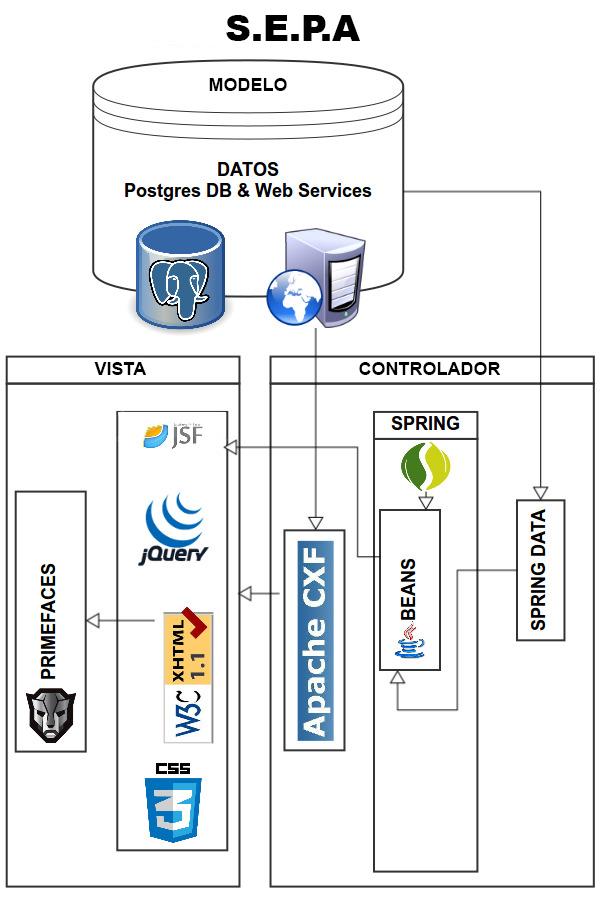
\includegraphics[scale=0.6,angle=0]{images/diagrama.jpg}
\caption{Diagrama general del sistema}
\label{Diagrama general del sistema}
\end{center}
\end{figure}
\chapter{Marco Teórico}
\thispagestyle{empty}
\section{Base Conceptual}
\subsection{Establecer el problema}
En la Universidad existe la necesidad de disponer de información relevante para apoyar la toma de decisiones, esta información debe ser respaldada por enormes volúmenes de registros que se guardan constantemente en el sistema DirDoc de la Universidad. Para este propósito existe el Sistema Estadístico de Profesores y Alumnos (SEPA), el cual incluye indicadores que pueden ser usados para el estudio de la institución. Con el tiempo la cantidad de datos va en crecimiento, también crece la cantidad de información y la necesidad de actualizar y modificar las tablas de manera más rápida y sencilla.

A raíz de esto se generaron ciertos problemas que comprometen la integridad de la data y por tanto entorpecen el objetivo inicial de SEPA, estos son:

\begin{enumerate}
	\item Inserción de data en SEPA, mediante la planificación con funcionarios de la universidad, se solicita la inserción de data desde DirDoc hacia SEPA, lo que origina muchos problemas, como el tiempo que se ocupa en este proceso, la alta probabilidad de falla debido a un error humano en varios puntos del proceso.
	\item Lentitud: Debido a que el sistema anterior SEPA estaba construido con PHP, el cual es una herramienta flexible pero de compleja mantención. Se hace poco eficiente su uso a medida que la cantidad de data va creciendo.
	\item Insuficiente: Debido a que no existe un modulo de actualización de data.
	\item No existe un mecanismo de diferenciación de usuarios. Haciendo este sistema un tanto inseguro, ya que no debiera existir la posibilidad de mirar toda la data, si no solo una parte, en relación a un perfil.
	\item Data corrupta o inexistente: Con el paso del tiempo la data se torna corrupta, poco actualizada o simplemente no existe.
\end{enumerate}
\subsection{Oportunidad de mejora}
La solución que otorga este proyecto es la creación de varios servicios web que proveen datos que deben ser procesados y mantenidos en una base de datos local. Este sistema debe validar la integridad de los datos evitando perdida de registros. A continuación se desarrolla un Mantenedor de los datos que componen el sistema, en el cual es posible buscar registros, comprobar que estén correctos y si no lo están, poder modificarlos.
\subsection{Uso de Java}
Esta actualización es construida a través del compendio de tecnologías que engloba la convención JavaEE (Java Enterprise Edition), caracterizada por un enfoque estandarizado en el proceso productivo, lo que permite automatizar varios procesos y centrarnos en el proyecto. Esto facilita la construcción del mismo de manera más estable y segura. Agregando valor mediante la incorporación de distintas herramientas, explicadas en este documento, que posibilitan un desarrollo de calidad y mejorable en el futuro.
\subsection{Desventaja de PHP}
Algunas tecnologías como PHP permiten crear la página de manera rápida e incorporar un framework de persistencia, pero son difíciles de escalar y mantener. Otros frameworks como Ruby on Rails podrían llevar a cabo esta tarea de mejor manera, pero el punto frágil es su curva de aprendizaje que es bastante alta.

Esto nos lleva a tomar la decisión de abandonar PHP ya que lo que se busca es, una herramienta que tenga reusabilidad en la organización y capacidad de mejora, manteniendo la robustez y la simpleza.
% enfocar a las cosas que no se pueden haceren otros lenguajes.
\section{Ciclo de vida del Software}
\begin{enumerate}
\item Toma de requerimientos: Proceso que básicamente comprende 2 actividades, primero, la toma de requerimientos en base al sistema SEPA anterior, segundo, una serie de entrevistas para captar las historias de usuarios que posteriormente se convierten en requerimientos.
\item Análisis de requerimientos: Etapa en donde el profesor encargado discute con el alumno los requerimientos que deben realizarse, de acuerdo con las expectativas y las necesidades del equipo de trabajo.
\item Diseño de la solución: Proceso en donde se desarrolla el modelo de datos que debe soportar a los requerimientos, y las interfaces asociadas.
\item Diseño estructural: En este punto el alumno trabaja desarrollando el proyecto en coordinación con el profesor encargado y éste va revisando constantemente el avance, emitiendo calificaciones y aclaraciones.
\item Pruebas: Proceso por el cual el profesor encargado verifica la fiabilidad y calidad de los requerimientos ya resueltos.
\item Instalación: En este punto se produce la incorporación del sistema en su ambiente por defecto, lo que implica un término del proyecto, solo dentro del marco de Trabajo de título para el alumno.
\end{enumerate}

Desde esta perspectiva cada componente que se quiera agregar al proyecto, debe obligatoriamente partir desde el Análisis de requerimientos, pasando por un Diseño de la solución, para después llegar al Diseño estructural y Pruebas, para finalmente Instalar los cambios.

\begin{figure}[!hbp]
\begin{center}
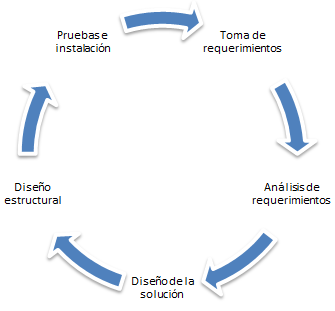
\includegraphics[scale=0.6,angle=0]{images/cicloMini.PNG}
\caption{Ciclo de vida}
\label{Organigrama de rectoria}
\end{center}
\end{figure}
%imagen de como tiene que ser
\section{Estado del arte}
La calidad de datos que se obtienen en un establecimiento educacional, es de vital importancia para la planificación y desarrollo de sus actividades, ya que permiten una adecuada toma de decisiones que afectan el desarrollo de la institución, ya sea de forma docente como administrativa. 

Los estudios estadísticos son tambien importantes porque entregan retroalimentación y permiten una visión más clara de la realidad operativa.

Las instituciones educacionales que forman profesionales deben estar evaluadas por organismos preparados en auditar las características de su desempeño. Para estos efectos, existen organismos estatales que acreditan lo que cada Universidad propone, pero por otro lado existen entandares de calidad que son medidos por organismos extranjeros, para dar un sello de calidad, evaluando a partir de datos estadísticos  \cite{data1}.

Un ejemplo en el mercado de un proyecto similar a este trabajo de título es: En 2009 se abre el sitio QS Top Universities que hasta el día de hoy es un sitio altamente eficiente en evaluación mediante ránkings enfocados a entregar información a organismos y personas relacionadas con post-grados, MBA, estudios de ingeniería y negocios, desarrollando estadísticas de alto alcance en sitios web, eventos, guías y programas por Internet y finalmente entregando soluciones técnicas a otros organismos, tales como Universidades o empresas privadas, entre otras.

Sus datos manejan información de 41 países, entre los que están: Argentina, Ecuador, Japon, Singapur, Australia, Egipto. Su servicio es sin costo para todo el público y permite un tipo de suscripción gratuita para visualizar tablas comparativas de manera simple.

Permite hacer comparaciones por categorías varias, ya sea país, estado, ciudad y otras características internas de la Universidad como ponderaciones o prestaciones de alumnos, tales como cantidad de alumnos o la segregación por sexo o etnia en cada localidad.

Su objetivo general es ser el principal sitio de ránkings de educación.

Una debilidad de este sistema es que solo hace comparaciones de carácter global y no se involucra en temas más finos sobre cada Universidad, solo maneja datos recopilados de otras investigaciones para completar este tema.

QS Top Universities es una empresa de tamaño mediano, con más de 150 empleados en oficinas de todo el mundo. También se realizan Tours en 70 ciudades en 39 países que permiten a más de 50.000 espectadores, los cuales buscan entrar a una Universidad  \cite{data2}.

Otro ejemplo es el Ránking de Calidad de las Universidades Chilenas, es un trabajo realizado por AméricaEconomía Intelligence en el 2010, un sitio de ránking para instituciones educacionales en Chile, que utiliza ciertos criterios, como son la cantidad de investigaciones o la masa de estudiantes que entran en cada Universidad.

%Algunos datos generales que se obtienen, son que la Universidad de Chile y la PUC, tienen diferencias muy pequeñas %en el campo de la investigación, para lo cual se mostró que la Universidad de Chile aporto con 1.329 papers %publicados, en cambio la PUC hizo un aporte total de 1.029 publicaciones.

Mucha de esta data estadística es recopilada a traves de encuestas enviadas a distintas Universidades y organismos de educación en Chile. Cada institución trabaja con esto, con el fin de captar publico que desea tomar una decisión en el mercado.

Este sistema da cuenta de una necesidad por parte de las Universidades, de ser más competitiva en el mercado universitario. Aumentando los esfuerzos por recibir más estudiantes, mostrando mejores profesores, alumnos e investigaciones.

La gran debilidad de este sistema es que no se muestran muchos criterios de comparación y solo da una arista para comparar lo que resulta insuficiente para formarse una opinión global del sistema.

Finalmente se observa a las Universidades actuales buscando organismos extranjeros capaces de certificar las características de la educación que ofrecen, de esta manera muestran no solo una acreditación por un organismo chileno, sino también una necesidad de competir a nivel internacional \cite{data3}.

%\section{Justificación del Trabajo de título}
%La UTEM requiere un sistema informático que agregue funcionalidades para el control de sus datos de manera simple y segura. En el anterior SEPA los datos eran extraídos directamente del DirDoc, dando la posibilidad de cometer errores de inserción graves. Con este nuevo sistema, ahora no solo hay una seguridad con los datos que son transferidos desde servicios web, sino que también implementa un Sistema de Autenticación, gracias a su sistema de perfiles de usuarios que limita el acceso en el sitio para más de 2 tipos de usuarios.

%El avance gracias al servicio web es justificado con las siguientes mejoras que se tienen que hacer para que esta modificación se pueda realizar:

%\begin{itemize}
%	\item Sistema de comunicación desde DirDoc hacia SEPA: Programar distintas interfaces que entregan información a SEPA, pasando por todos los requerimientos que se puedan originar, y dejando paso a futuras peticiones por parte de este sistema a DirDoc.
%	\item Sistema de rastreo de data y corrección: Programar un mecanismo que detecte cuando se presenten problemas con la data, ya sea que venga corrupta o mal formada, convirtiéndola en data en blanco, para posteriormente poder ser reparada.
%	\item Sistema de inserción de data a un modelo estructurado para funcionar con JPA: Generar un modelo de datos que permita la interacción frente al patrón Modelo, Vista, Controlador, en donde el modelo es la estructura simple de la data, pero permite tomar todos los conjuntos de data de manera fácil, rápida y óptima.
%	\item Sistema cronométrico de petición de data a DirDoc: Programar un sistema que haga las distintas consultas a DirDoc de manera cronometrada, ocupando distintos horarios para hacer las ejecuciones. Por ejemplo haciendo que las ejecuciones sean en un horario en que poca gente hace uso de los servicios. Minimizando los recursos.
%\end{itemize}

%Por otro lado la creación del sistema mantenedor comprende las siguientes mejoras:

%\begin{itemize}
%	\item Inserción de perfiles de usuario: Programar por medio de herramientas dentro de JavaEE, distintos perfiles que serán capaces de mirar en ciertas medidas la data que ofrece el sistema.
%	\item Mejora de la interfaz de usuario: Programar componentes que el usuario pueda aprender a usar de forma rápida y eficiente.
%	\item Uso completo de las tablas de SEPA: Mediante los distintos perfiles es posible llegar a todas las tablas, lo que supone el mantenimiento de todas estas.
%	\item Visualización y mantenimiento de las tablas: Programar sistema de mantenimiento para todas las tablas que un usuario pueda visualizar
%\end{itemize}

\section{Análisis de las herramientas}
El desarrollo de las aplicaciones debe ser con un lenguaje que nos permita la correcta ejecución de las tareas de diseño y desarrollo. Por lo cual resulta interesante desarrollar algunos criterios que nos mostrarán las características y la justificación de nuestra elección a la hora de pensar en un lenguaje apropiado para este proyecto.

\begin{enumerate}

\item Sencillez: Característica del lenguaje que hace que sea fácil el crear o entender el código, al momento de programarlo o leerlo \cite{data4}.

\item Robustez: Capacidad interna del lenguaje de proporcionar herramientas que permiten minimizar los errores producidos por el programador \cite{data4}.

\item Seguridad: Característica que hace que un lenguaje no permita tocar accesos a donde la aplicación no debiese ir (en la mayoría de los casos), ejemplos, restringir accesos, ejecución de pruebas o derechos de accesos \cite{data4}.

\item Portabilidad: Capacidad de un lenguaje para correr en múltiples sistemas operativos \cite{data4}.

\item Neutralidad: Independencia de la maquina en donde se ejecuta, concibiendo una experiencia lo más similar posible entre distintas máquinas y sistemas operativos \cite{data4}.

\item Interfaz: Capacidad de producir fácilmente interfaces cómodas para el usuario final \cite{data4}.

\item Expresividad: Capacidad de minimizar el número de líneas con las que una acción puede ejecutarse dentro del código \cite{data5}.

\item Compilación: Capacidad de minimizar el tiempo que toma poder compilar el código producido.

\item Aprendizaje: Dificultad para aprender el lenguaje. Basado simplemente en la experiencia propia sobre cada lenguaje.

\item Estructuras de control: Un lenguaje debe proveer estructuras simples de control, pero tampoco llenarse de estructuras que nunca se van a utilizar \cite{data6}.

\item Abstracción: Capacidad de convertir cosas difíciles en algo simple con la estructura del lenguaje \cite{data6}.

\end{enumerate}

También es importante tener en cuenta el lenguaje a utilizar en el momento de la creación del proyecto, de esta manera se pondrán los lenguajes candidatos: PHP, .NET, Ruby on Rails y Java. Ver anexo.

En la siguiente tabla se muestra una comparación de las cuatro tecnologías anteriormente presentadas de forma explicita para comprender nuestra elección. Es importante señalar que uno de los aspectos que marca profundamente la elección sobre el lenguaje con que se va a realizar este proyecto, es determinada por los conocimientos que tiene el alumno y las indicaciones del profesor, en pos de realizar lo más rápido posible el trabajo, haciéndolo de forma elegante. 

\begin{table}
\begin{tabular}{| l | l | l | l | l |}
\hline
 & 
\includegraphics[scale=0.08]{images/icons/php.png} & 
\includegraphics[scale=0.08]{images/icons/net.png} & 
\includegraphics[scale=0.51]{images/icons/ruby-on-rails.png} & 
\includegraphics[scale=0.1]{images/icons/java.png}\\
\hline
\textit{Sencillez} & \textcolor{green}{\CheckmarkBold} &  \textcolor{red}{\XSolidBold} &  \textcolor{red}{\XSolidBold} & \textcolor{green}{\CheckmarkBold}\\
\hline
\textit{Robustez} & \textcolor{red}{\XSolidBold} & \textcolor{green}{\CheckmarkBold} & \textcolor{green}{\CheckmarkBold} & \textcolor{green}{\CheckmarkBold}\\
\hline
\textit{Seguridad} & \textcolor{red}{\XSolidBold} & \textcolor{red}{\XSolidBold} & \textcolor{green}{\CheckmarkBold} & \textcolor{green}{\CheckmarkBold}\\
\hline
\textit{Portabilidad} & \textcolor{green}{\CheckmarkBold} & \textcolor{red}{\XSolidBold} & \textcolor{red}{\XSolidBold} & \textcolor{green}{\CheckmarkBold}\\
\hline
\textit{Neutralidad} & \textcolor{green}{\CheckmarkBold} & \textcolor{red}{\XSolidBold} & \textcolor{green}{\CheckmarkBold} & \textcolor{green}{\CheckmarkBold}\\
\hline
\textit{Interfaz} & \textcolor{red}{\XSolidBold} & \textcolor{green}{\CheckmarkBold} & \textcolor{green}{\CheckmarkBold} & \textcolor{green}{\CheckmarkBold}\\
\hline
\textit{Expresividad} & \textcolor{green}{\CheckmarkBold} & \textcolor{red}{\XSolidBold} & \textcolor{green}{\CheckmarkBold} & \textcolor{red}{\XSolidBold}\\
\hline
\textit{Compilación} & \textcolor{green}{\CheckmarkBold} & \textcolor{red}{\XSolidBold} & \textcolor{green}{\CheckmarkBold} & \textcolor{red}{\XSolidBold}\\
\hline
\textit{Aprendizaje} & \textcolor{green}{\CheckmarkBold} & \textcolor{red}{\XSolidBold} & \textcolor{green}{\CheckmarkBold} & \textcolor{green}{\CheckmarkBold}\\
\hline
\textit{E. de control} & \textcolor{green}{\CheckmarkBold} & \textcolor{green}{\CheckmarkBold} & \textcolor{green}{\CheckmarkBold} & \textcolor{green}{\CheckmarkBold}\\
\hline
\textit{Abstracción} & \textcolor{green}{\CheckmarkBold} & \textcolor{red}{\XSolidBold} & \textcolor{red}{\XSolidBold} & \textcolor{green}{\CheckmarkBold}\\
\hline
\textbf{Total} & 8 & 3 & 8 & 9\\
\hline
\end{tabular}
\caption{Información obtenida desde el trabajo con distintas herramientas}
\end{table}
Como lo muestra la tabla anterior, java cumple más criterios, en el sentido de la observación y el criterio subjetivo del alumno que realiza el trabajo.

\section{Criterios de Calidad}

Se mostrarán a continuación los criterios de calidad del proyecto. Estos criterios muestran de forma justificada, que la mejor elección es la que nosotros proponemos para la organización, pensando en los costes de tiempo y recursos económicos que un proyecto de esta clase puede significar.

\begin{enumerate}

\item Mantenibilidad: Característica que hace que nuestro proyecto sea fácil de corregir en caso de fallos. Basándose en la concepción de que un proyecto que tiene un modelo bien establecido es más fácil de reparar \cite{data11}.

\item Flexibilidad: Característica que indica la capacidad de agregar cambios, incluyendo también el hecho de que como es un sistema hecho dentro del contexto de esta Universidad está lo suficientemente enfocado en ella, pero también es posible cambiar algunas cosas en pos de que este sistema funcione también en otras Universidades. \cite{data11}.

\item Testeabilidad: Esto nos muestra que el modelo del sistema ha pasado por un test antes de ser ocupado en el proyecto. \cite{data11}.

\item Portabilidad: Ya que como se trabaja con Java, el proyecto es básicamente portable a casi cualquier tipo de sistema operativo, lo que lo hace un ente fácil de cambiar en otros entornos de trabajo y es perfectamente acomodable en ese sentido. \cite{data11}.

\item Integridad: Este sistema se caracteriza por su integridad con los datos, lo que nos muestra un dedicado trabajo sobre el tema de la base de datos. \cite{data11}.

\item Rapidez: El sistema está hecho de tal manera que debe funcionar de forma expedita y veloz, sobre todo con la enorme cantidad de datos que se van a manejar. \cite{data11}.

\end{enumerate}

\section{Patrones de Diseño}
Son arquitecturas estandarizadas para el desarrollo de software, permiten a los proyectos ser resueltos con estrategias ya probadas y que funcionan en la mayoría de los casos. Existen muchos patrones distintos, para este proyecto se utilizan todos los que se explican a continuación:

\begin{enumerate}

\item MVC, Modelo Vista Controlador: Establece que el software tiene por lo menos 3 capas de desarrollo las cuales son; modelo, donde se encuentran el acceso a datos como de una base de datos, ficheros o servicio web; vista, la parte del programa que interactúa con el usuario final; controlador, el código en donde esta el negocio que procesa los datos del modelo para posteriormente mostrarlos en la vista \cite{data22}. En SEPA se utiliza JSF, que es una tecnología que permite generar vistas para el usuario de forma ágil para los desarrolladores, permitiendo la separación de los objetos encargados de interpretar el patrón MVC.

\item SOA, Arquitectura orientada a servicios: Establece el software enfocado a los procesos de negocio, teniendo distintas capas de aplicaciones como: Aplicaciones básicas, caracterizadas por ser pequeñas y geográficamente establecidas; Exposición de Funcionalidades, donde rigen servicios; Integración de servicios, para intercambio de datos; Composición de procesos, determina términos de negocio y funcionalidades; Entrega, para usuarios finales \cite{data23}. Este proyecto hace uso de CXF que permite la integración de servicios entre procesos distintos. Mediante el uso de servicios web, conocidos por ser mecanismos de comunicación mediante un protocolo establecido, generando una arquitectura de servicios.

\item POA, Programación Orientada al Aspecto: Es un paradigma de programación relativamente reciente cuya intención es permitir una adecuada modularización de las aplicaciones y posibilitar una mejor separación de incumbencias. Con esto se pueden encapsular los diferentes conceptos que componen una aplicación en entidades bien definidas, eliminando las dependencias entre cada uno de los módulos. De esta forma se consigue razonar mejor sobre los conceptos, se elimina la dispersión del código y las implementaciones resultan más comprensibles, adaptables y reusables \cite{data24}. Para utilizar los servicios automáticos se hace uso de Spring, una tecnología que ocupa el criterio de aspecto para configurar funciones u operaciones, disminuyendo la cantidad de código que se usa para similares tareas.

\item DAO, Objeto de Acceso a datos: es un componente de software que suministra una interfaz común entre la aplicación y uno o más dispositivos de almacenamiento de datos, tales como una Base de datos o un archivo. El término se aplica frecuentemente al Patrón de diseño Object. Los Objetos de Acceso a Datos son un Patrón de los subordinados de Diseño Core J2EE y considerados una buena práctica. La ventaja de usar objetos de acceso a datos es que cualquier objeto de negocio (aquel que contiene detalles específicos de operación o aplicación) no requiere conocimiento directo del destino final de la información que manipula \cite{data25}. El modelo de datos de SEPA es consultado con JPA, que permite el acceso a los datos, de una forma genérica y lógica, facilitando el desarrollo, integrándose con Spring y JSF.

\end{enumerate}

\chapter{Integrador}
\thispagestyle{empty}

\section{Preámbulo}
A continuación se presenta el módulo de integración. Se explica el funcionamiento general de este. Cada uno de sus servicios son expuestos de manera ordenada y funcional.

\section{Funcionalidad}

El modulo de integración que se le agrega a SEPA es una herramienta de poca complejidad, en donde es posible hacer cargas de datos, que serán explicadas posteriormente. Además de esto existen herramientas que hacen posible las peticiones de información desde el módulo integrador hacia DirDoc, esta funcionalidad se carga por tareas determinadas en ciclos de tiempo predefinidos, que son explicados a continuación.

\section{Poblador}
Al proceso SEPA se le agrega un módulo integrador que permite la comunicación entre los datos del sistema de notas y estudiantes existente dentro de la Universidad (DirDoc). El fin de ésto es preguntar por datos que posteriormente serán insertados en las tablas del sistema nuestro. Para esto se utiliza a un Web Service que provee una interfaz en donde se obtiene la información, ésta posteriormente se normaliza y adecua a nuestro sistema y finalmente se persiste. Existen varios procesos de integraciones, cada uno va dirigido a un objeto que se quiere poblar.
\section{Web Service}
Es una tecnología que permite la comunicación entre 2 programas mediante un sistema que expone un protocolo para el traspaso de datos, donde el encargado de generar las preguntas debe tener información consistente y poder establecer la conexión. Por otro lado los programas se relacionan gracias a un meta lenguaje basado en XML (de etiquetado) que describe el código que debe implementarse para poder realizar las consultas y retornar objetos con los cuales posteriormente opera.

Eso es posible gracias a que se hace uso del framework Apache CXF que nos abstrae de la complejidad de programar un servicio web y nos permite realizar esta tarea de manera fácil. CXF nos pide información relacionada con la dirección del servicio a consumir y él se encarga de traernos las respuestas que necesitemos.

\section{Periodicidad}
Los procesos integradores de SEPA, funcionan bajo el esquema de periodicidad, siendo ejecutados en lapsos de tiempo y en un orden concreto. Esto quiere decir que ciertas tareas son ejecutadas una ves en el día, mientras que otras son ejecutadas una ves a la semana o al mes. También es posible configurar los horarios de ejecución, para poder ejecutarlos en momentos de poco flujo de datos.

\section{Operaciones}
La integración se basa en distintas operaciones separadas por el momento y la hora en donde se realizan, todas las tareas tienen el objetivo de poblar los datos propios por lo cual el trabajo de mapeo de datos es siempre distinto para todas las consultas y objetos que se tienen.
\subsection{Tarea diaria}
Tareas que se ejecutan una vez al día, en donde podemos encontrar: Actualizar Cohortes y Actualizar Estudiantes. El proceso obtiene los datos, principalmente, del servicio web llamado servicio carrera.
\subsection{Tarea semanal}
Tareas que se ejecutan una vez a la semana, en donde podemos encontrar: Actualizar Asignaturas Cursadas. El proceso obtiene los datos, principalmente, del servicio web llamado servicio curso.
\subsection{Tarea mensual}
Tareas que se ejecutan una vez al mes, en donde podemos encontrar: Actualizar Asignaturas Mallas, Actualizar Cursos, Actualizar Docentes y Actualizar Cargos. El proceso obtiene los datos, principalmente, del servicio web llamado servicio curso y docente.
\subsection{Tarea trimestral}
Tareas que se ejecutan cada tres meses, en donde podemos encontrar: Actualizar Asignaturas, Actualizar Cupos Carreras, Actualizar Titulados. El proceso obtiene los datos, principalmente, del servicio web llamado servicio utem y curso.
\subsection{Tarea semestral}
Tareas que se ejecutan cada semestre, en donde podemos encontrar: Actualizar Establecimientos y Actualizar Mallas. El proceso obtiene los datos, principalmente, del servicio web llamado servicio curso y estudiante.
\subsection{Tarea anual}
Tareas que se ejecutan una vez al año, en donde podemos encontrar: Actualizar Carreras, Actualizar Planes de Estudio y Actualizar Quintalización. El proceso obtiene los datos, principalmente, del servicio web llamado servicio curso, docente, utem y carrera.

\chapter{Mantenedor}
\thispagestyle{empty}
\section{Preámbulo}
A continuación se presenta el módulo de mantenedor. Se explica el funcionamiento general de este. Cada uno de sus componentes son explicados, validando su facilidad y simpleza.
\section{Introducción}

El mantenedor es la interfaz nueva que tiene SEPA después de estas mejoras, es la parte que el usuario final apreciará de manera distinta, ya que ahora se tienen perfiles, visualización e incluso modificación de data. De manera lógica y simple, manteniendo siempre la facilidad del desarrollo para futuros componentes.

\section{Sitio Web}
El proyecto mantenedor es un sitio web que utiliza la tecnología Java Server Faces o (JSF), que permite la visualización de una estructura de código en formato xml para mostrar sitos web con contenido dinámico en java. Sobre esta tecnología se ocupa Primefaces enriqueciendo las características de JSF proporcionando componentes HTML complejos (tales como menús despegables o tablas con distintas funcionalidades ya programadas).
\section{Ingreso}
El ingreso al sitio se hace con usuario y contraseña, cada usuario esta asociado a un perfil que limita el uso en el sitio, la autentificación esta hecha con Spring Security, un framework que permite automatizar el paso de perfiles con sus contraseñas, gestionando la encriptación y la desencriptación, de esta manera los ingresos al sitio son seguros, manejando los distintos tipos de roles.

También el inicio de la página cuenta con links hacia sitios de interés que están dentro de la Universidad.
\section{Mantenedores}
Al ingresar al sitio uno puede ver un menú con los distintos mantenedores, abajo se ve un registro con los ingresos al sitio e información detallada con algún indicador.

Volviendo al menú tenemos una serie de opciones:

\begin{itemize}
	\item Inicio: Que nos da un mensaje de bienvenida y es un punto de partida.
	\item Acceso: Contiene los mantenedores de Acceso, Auditoría, Rol y Usuario.
	\item Geografía: Contiene los mantenedores de País, Región, Provincia y Comuna.
	\item UTEM: Contiene los mantenedores de Facultad, Departamento, Escuela, Contrato, Docente, Jerarquía, Jornada, Carrera, Asignatura Malla, Cupo Carrera, Malla, Plan de Estudio y Requisito de Asignatura.
	\item Curso: Contiene los mantenedores de Asignatura, Asignatura Cursada, Curso, Estado de Asignatura y Régimen.
	\item Estudiante: Contiene los mantenedores de Establecimiento, Grupo Dependencia, Rama, Régimen Educacional, Tipo Establecimiento, Cohorte, Egresado, Estado Alumno, Estudiante, Histórico Alumno, Tipo de Ingreso y Titulado.
	\item Contacto: Contiene los mantenedores de Contacto y Preguntas Frecuentes.
	\item Sesión: Que tiene el Logout para poder salir del sistema cerrando sesión.
\end{itemize}

Todos estos mantenedores cumplen con las mismas funciones de buscar, borrar, filtrar, agregar y modificar los registros en cada una de las tablas que uno elija.
\chapter{Evaluación de Costos}
\section{Métodos de estimación}
Una forma de estimación es el Modelo Constructivo de Costos, llamado COCOMO el cual proporciona herramientas matemáticas para definir el valor final de un proyecto. Es un proceso que gana fuerza con proyectos que van creciendo a medida que se van desarrollando, por lo cual esta orientado a la estimación de lo que es el producto final. Sus inconvenientes son que sus resultados no son proporcionales a la cantidad de tareas que el proyecto cumple. Lo que obliga siempre a modificar sus valores para obtener un resultado concreto. Este proceso particularmente mide el tamaño 
del proyecto, pero no su funcionalidad.

Finalmente se elije el sistema de Puntos de Función, el cual es un proceso que toma fuerza en el impacto de cada componente realizada, donde cada pieza de desarrollo es un punto a sumar en el calculo final. Esta enfocado a los distintos tipos de desarrollo que uno debe hacer en un proyecto, utilizando una categorización de tal manera que se tiene en cuenta el impacto en conjunto de todas estas piezas. Al igual que COCOMO utiliza una función matemática para despejar el valor monetario final, pero su calculo es menos estimado y esta sujeto a una regla mas firme.
\section{Puntos de Función}
Para evaluar los costos monetarios de este proyecto se utilizara el cálculo de Puntos de Función para llegar a un valor justificado. Mediante una función matemática que utiliza varios parámetros, divididos en 2 ramas. Este método de medición del software es un extracto de las practicas establecidas por la IFPUG (Grupo de usuarios internacional función Point), que se encarga de definir los costos de proyectos que son ocupados a nivel mundial.

\section{Conteo de puntos}

\begin{enumerate}
	\item Ficheros Internos Lógicos (FIL): Este valor representa la cantidad de información de los datos internos, contenida en bases de datos y ficheros de configuración, por lo tanto se tomará como valor final la cantidad de tablas contenidas en el modelo. Su valor de complejidad es 8, ya que es una tarea que puede ser difícil en un comienzo, pero luego es repetitiva.
	\item Ficheros Externos de Interfaz (FEI): El proyecto utiliza datos externos que son administrados por la aplicación DirDoc. Por ejemplo hay un aproximado de 32 servicios adjuntos al modelo, contenidos en 11 servicios, mas, un aproximado de 24 sub-tareas externas en el integrador contenidas en 6 tareas grandes. Es una tarea simple, al cual se le asigna el valor 3.
	\item Entrada Externa (EE): El sistema consume servicios web provenientes de otros sistemas. Su valor es 6, ya que es difícil en un comienzo.
	\item Salida Externa (SE): El sistema muestra la totalidad de los datos internos en su parte visual. En este caso particular todas las tablas del modelo tienen un apartado visual en la vista. Su valor es 8 ya que es una tarea compleja en un comienzo.
	\item Consulta Externa (CE): El sistema tiene mantenedores de todos sus datos en base de datos, para poder ser modificables por los usuarios. Su valor es 8 debido a que son alrededor de 30 mantenedores y es una tarea delicada.
\end{enumerate}

\begin{table}
\textbf{Tabla de valores ponderados}\\
\begin{tabular}{| l | l | l | l |}
\hline
\textbf{Característica} & \textbf{Ponderación} & \textbf{Valor} & \textbf{Determinante ponderado} \\
\hline
FIL & 49 & medio & 8\\
\hline
FEI & 43 & medio & 3\\
\hline
EE & 16  & alto  & 6\\
\hline
SE & 43  & alto  & 8\\
\hline
CE & 43  & alto  & 8\\
\hline
\end{tabular}
\caption{Tabla de valores ponderados}
\end{table}
Los parámetros anteriores deben ser convertidos en distintas tablas.
\begin{table}
\textbf{Complejidad de los ficheros}\\
\begin{tabular}{| l | l | l | l |}
\hline
\textbf{RET/DET} & \textbf{1-19} & \textbf{20-50} & \textbf{51+} \\
\hline
1 & Bajo & Bajo & Medio\\
\hline
2-5 & Bajo & Medio & Alto\\
\hline
6+ & Medio & Alto & Alto\\
\hline
\end{tabular}
\caption{Complejidad de los ficheros}
\end{table}
\begin{table}
\textbf{Complejidad de las entradas}\\
\begin{tabular}{| l | l | l | l |}
\hline
\textbf{FICH/DET} & \textbf{1-4} & \textbf{5-15} & \textbf{16+} \\
\hline
0-1 & Bajo & Bajo & Medio\\
\hline
2 & Bajo & Medio & Alto\\
\hline
3+ & Medio & Alto & Alto\\
\hline
\end{tabular}
\caption{Complejidad de las entradas}
\end{table}
\begin{table}
\textbf{Complejidad de las Salidas}\\
\begin{tabular}{| l | l | l | l |}
\hline
\textbf{FICH/DET} & \textbf{1-5} & \textbf{6-19} & \textbf{20+} \\
\hline
0-1 & Bajo & Bajo & Medio\\
\hline
2-3 & Bajo & Medio & Alto\\
\hline
4+ & Medio & Alto & Alto\\
\hline
\end{tabular}
\caption{Complejidad de las salidas}
\end{table}
\begin{table}
\textbf{Tabla de valores calculados}\\
\begin{tabular}{| l | l | l | l | l |}
\hline
\textbf{TIPO} & \textbf{Bajo} & \textbf{Medio} & \textbf{Alto} & \textbf{Total} \\
\hline
EE & x3  & \textbf{8x4}  & x6 & 32\\
\hline
SE & x4  & \textbf{3x5}  & x7 & 15\\
\hline
CE & x3  & x4  & \textbf{6x10} & 60\\
\hline
FIL & x7 & x10 & \textbf{8x25} & 200\\
\hline
FEI & x5 & x7 & \textbf{8x15} & 120\\
\hline
TOTAL &  &  & & 427\\
\hline
\end{tabular}
\caption{Tabla de valores calculados}
\end{table}

\section{Características generales del sistema}

En esta sección se evalúa con un número de 0 a 5 las distintas características que este sistema puede o no tener, y finalmente se ponderan para generar un valor que nos permite hacer el ajuste para el conteo de puntos anterior.

\begin{enumerate}
	\item Comunicación de Datos: [4 puntos] Varios teleprocesos pero con el mismo protocolo de comunicaciones. Tiene una dificultad de programación media, por que es un proceso repetitivo.
	\item Proceso Distribuido: [4 puntos] Proceso de datos distribuidos y transferencia de datos en línea en ambas direcciones. Por ejemplo una red de cajeros automáticos en donde estos procesan parte de la transacción. Tiene una dificultad de programación media por que es solo un proceso complejo.
	\item Objetivos de Rendimiento: [4 puntos] Se utilizan herramientas de análisis de rendimiento durante el diseño, desarrollo e instalación, con el objetivo de alcanzar el rendimiento demandado por el usuario. Tiene una dificultad de programación media, debido a se ocupan componentes que facilitan el desarrollo.
	\item Configuración de Explotación Usada intensamente por Otros Sistemas: [1 punto] Existen restricciones, pero son las usuales de cualquier equipo departamental. No es necesario hacer consideraciones especiales. Tiene una dificultad de programación baja. 
	\item Tasa de Transacciones: [2 puntos] Se prevén peaks de operaciones semanales. Tiene una dificultad de programación baja.
	\item Entrada de datos EN-LÍNEA: [5 puntos] La entrada de datos interactivas superan el 30 por ciento de las transacciones. Tiene una dificultad de programación alta, ya que problemas en el código pueden generar tiempos de respuesta altos.
	\item Eficiencia con el Usuario Final: [3 puntos] Seis o más factores, pero sin especiales requerimientos de eficiencia. Tiene una dificultad de programación media.
	\item Actualizaciones EN-LÍNEA: [4 puntos] Protección ante pérdidas y el sistema se ha de diseñar e implementar con estas consideraciones. Tiene una dificultad de programación media.
	\item Lógica de Proceso Interno Compleja: [5 puntos] La aplicación llevará incorporados sistemas de seguridad y control. Tiene una dificultad de programación alta, ya que es un proceso que requiere un tipo de seguridad.
	\item Reusabilidad del Código: [5 puntos] La aplicación ha sido específicamente empaquetada y/o documentada para ser fácil de reutilizar. Tiene una dificultad de programación alta, debido a que se debe programar de manera elegante y permitiendo implementaciones futuras.
	\item Contempla la Conversión y Facilidad de Instalación: [0 puntos] No reemplazamos un sistema existente o no se requiere conversión. Tampoco se enuncia nada sobre la instalación.
	\item Facilidad de Operación: [5 puntos] Sistema automático sin intervención humana. Tiene una dificultad de programación alta, ya que es nesesario programar muchos componentes para que el sistema sea automático.
	\item Instalaciones Múltiples: [3 puntos] La aplicación correrá en múltiples entornos de Hw o Sw y se tiene en cuenta desde la fase de diseño. Tiene una dificultad de programación media, debido a que es un proceso un poco largo el ajustarlo a múltiples ambientes.
	\item Facilidad de Cambios: [3 puntos] El cambio de la configuración se hace interactivamente y tiene efecto inmediato. Tiene una dificultad de programación media, por que la gestión de los cambios es proporcionada por el servidor.
\end{enumerate}
\begin{table}
\textbf{Cálculo de los puntos de función ajustados}\\
\begin{tabular}{| l | l | l |}
\hline
\textbf{No.} & \textbf{Factor de Complejidad} & \textbf{Valor}\\
\hline
1 &  Comunicación de Datos & 4 \\
\hline
2 &  Proceso Distribuido &4  \\
\hline
3 & Objetivos de Rendimiento  &4  \\
\hline
4 & Configuración Explotación Compartida  & 1 \\
\hline
5 & Tasa de Transacciones  & 2 \\
\hline
6 &  Entrada de Datos EN-LÍNEA &  5\\
\hline
7 & Eficiencia con el Usuario Final  &  3\\
\hline
8 & Actualizaciones En-LÍNEA  & 4 \\
\hline
9 & Lógica del Proceso Interno Compleja  &  5\\
\hline
10 & Reusabilidad del Código  &  5\\
\hline
11&  Contempla la Conversión e Instalación &  0\\
\hline
12& Facilidad de Operación  &  5\\
\hline
13& Instalaciones Múltiples  &  3\\
\hline
14& Facilidad de Cambios  & 3 \\
\hline
\multicolumn{2}{|c|}{Factor de Complejidad Total (FCT)} & 48\\
\hline
\end{tabular}
\caption{Cálculo de los puntos de función ajustados}
\end{table}

\section{Puntos de función ajustados}
La siguiente fórmula describe la cantidad ajustada de puntos de función y éstos a su vez son multiplicados por el valor en horas dando lo que cuesta en tiempo y dinero, cada uno de los puntos obteniéndose finalmente el valor ponderado del proyecto en sí.

\begin{math}
PFA=PFSA * ( 0.65 + ( 0.01 * FCT ) = 427 * ( 0.65 + ( 0.01 * 48 ) = 452.51
\end{math}

Donde se obtuvo un total de 452 puntos de función ajustados, los que vienen a ser puntos de cambios en el proceso de desarrollo, los cuales por lo menos requieren un proceso de medición para posteriormente pasar a la programación. Después se multiplican los Puntos de Función por un factor de 4 horas hombre, aproximadamente, por cada punto de función.

\begin{math}
452.51 PF * 4 (HH / PF) = 452.51 * (4) = 1810.04 HH
\end{math}

Finalmente se multiplican las horas hombre por el factor 1.2 UF / HH.

\begin{math}
1810.04 HH * 1.2(UF / HH) = 2172.048 UF = 54.213.601 \$
\end{math}

El proyecto tiene un costo mínimo de 50.000.000 pesos.

\chapter{Conclusiones}

\section{Metodología de Trabajo}
Las metodologías de trabajo utilizadas principalmente son, el desarrollo en cascada, en donde se tiene una serie de hitos a cumplir y a su vez se tiene un tiempo para desarrollarlos. La ventaja de trabajar de esta manera es que se tiene un calendario de actividades riguroso, la principal desventaja es que si hay problemas en el desarrollo hay que diseñar nuevamente el modelo de trabajo. Otra metodología utilizada es el Prototipado el cual indica que cada desarrollo nuevo es precedido de uno de carácter similar. Esto significa que en la mayoría de los casos, el programa se completa a medida que se van iterando un desarrollo general sobre muchos otros particulares que hacen uso del modelo genérico, el cual implementa una funcionalidad esperada por todo el conjunto de funciones realizadas.

\section{Garantías de calidad}
La calidad de este sistema se ve potenciada por varios aspectos, los cuales se explicarán a continuación:

\begin{enumerate}
        \item Uso de una base de datos PostgreSQL: Un sistema gestor de bases de datos, de código abierto, echo para ser una potente forma de mantener grandes cantidades de datos. Siendo un proyecto realizado de manera altruista por muchos desarrolladores a nivel mundial, es muy estable, seguro y es el entorno necesario para que el sistema SEPA trabaje sin necesidad de pensar en licencias u otros tipos de registros de datos. Contiene una infinidad de tipos de datos que fortalece la forma de como uno ingresa parámetros \cite{data18}.
        \item Uso de Mybatis: Herramienta de ayuda para sentencias SQL que permite el uso de cualquier base de datos, con gran escalabilidad y adaptabilidad, permitiendo escribir las consultas que uno desee ejecutar y mapearlas directamente en los objetos que uno desee. Tiene un nivel de complejidad medio, lo que hace que sea un poco difícil aprender, la incorporación de nuevos elementos de data es ordenada y escalable \cite{data19}.
        \item Uso de WebServices: Una tecnología que utiliza un conjunto de protocolos y estándares que sirven para intercambiar datos entre aplicaciones. Distintas aplicaciones de software desarrolladas en lenguajes de programación diferentes y ejecutadas sobre cualquier plataforma, pueden utilizar los servicios web para intercambiar datos en redes de ordenadores como Internet \cite{data20}.
        \item Uso de Primefaces: Una librería de componentes para JavaServer Faces (JSF) de código abierto que cuenta con un conjunto de componentes enriquecidos que facilitan la creación de las aplicaciones web. Soporte de ajax con despliegue parcial, lo que permite controlar qué componentes de la página actual se actualizarán y cuáles no \cite{data21}.
        \item Uso de Metodología de Trabajo: El uso de PSP fortalece el desempeño del proyecto, mostrando los errores que el proceso de desarrollo pueda presentar, desde esta perspectiva es necesario destacar que cuando se van anotando los errores éstos tienden a disminuir con el tiempo por lo que en las etapas finales es muy difícil encontrar errores en el desarrollo.
        \item Uso de Patrón de diseño: El patrón MVC ha hecho de este proyecto un ente robusto y consistente que puede ser mejorable incluso con poco conocimiento, ya que posee una base sólida que sustenta su funcionamiento, por lo cual los cambios que se puedan necesitar en el futuro harán uso de las herramientas que se fabricaron en el desarrollo mismo.
        \item Uso de Java y Frameworks: Esto nos permite una autonomía en varios aspectos, ya que nosotros como impulsores de proyectos tenemos siempre que velar porque todo el desarrollo sea altamente eficiente, y una manera muy clara de obtener eso es mediante el uso de herramientas que ya han sido muy probadas y se encuentran en uso de muchos otros proyectos. Dado que en otros sistemas esto ha funcionado muy bien es de esperar que en el nuestro también funcione de igual modo.
        \item Pruebas de rendimiento: Las pruebas sobrecargan el sistema de tal manera que nos permiten decir a ciencia cierta si el software es capaz de resistir lo que los datos nos entregan, y estas nos demuestran que el trabajo realizado cumple con ciertas características de un proyecto web de gran valor.
\end{enumerate}

Finalmente con estos puntos se puede tener una clara idea de la calidad del producto que se entrega, de cómo éste puede mejorar aún mas, e incluso cambiar y adecuase a otras necesidades.

\section{Conclusión Final}
El trabajo correspondiente al Sistema Mantenedor e Integrador en SEPA ha mostrado como recuperar datos que pueden ser difíciles de manejar. Los datos para este trabajo no estaban del todo bien organizados, esto quiere decir que cuando se observan, es posible encontrar insuficiencias de campos en los objetos mostrados en las tablas de los mantenedores, por lo cual están preparados para ingresar datos en los sectores que lo requieran.

También es posible identificar errores estructurales de información. Por ejemplo, en el sistema anterior entraban datos que contenían errores repetidos en todas las filas de ciertas tablas. En el nuevo sistema está preparado para resistir ese tipo de datos y cargar una data estándar que más adelante será reparada por el sistema Mantenedor.

Un proyecto de estas características es una importante oportunidad de mejoras, tales como: mantenibilidad de la data, aunque esta contenga errores, ya que es posible editar aspectos mínimos dentro de todas las tablas, conectividad con servicios web, manejado por parámetros SOAP, dejando la complejidad de las comunicaciones a frameworks que se encargan de trabajar con estas interacciones.

Gracias a este trabajo se puede hablar de indicadores estadísticos, los cuales nos proporcionan información que regulan el funcionamiento de cualquier organización. Para este caso en particular, el desarrollo de indicadores, nos permite sostener una organización a nivel de estudiantes, integrando consultas estadísticas a problemas particulares en estudiantes y profesores.

La ventaja de que este sistema se comunique con otros mediante el uso de WebServices es que a lo largo de la vida útil de este proyecto se pueden agregar otros proyectos que pueden nutriste de la información que SEPA produce.
\section{Trabajo Futuro}
Para ampliar las posibilidades de un trabajo que descansa sobre el valor de potenciar las capacidades administrativas de una institución académica, es necesario hacer estudios que posibiliten un mayor alcance de datos, tal como lo hace SEPA, por tal razón es de vital importancia promover nuevas mejoras que hagan de este sistema una herramienta completa en el desarrollo de las capacidades generales de una organización, como lo es la Universidad Tecnológica Metropolitana.

Se puede considerar el integrar un motor de minería de datos que revele información que hasta ahora no se ha obtenido dentro de los marcos de este proyecto, por ejemplo, una herramienta que obtenga formulaciones o métodos de aproximación para datos del futuro. Tal cosa produciría un impacto en SEPA ya que con esta perspectiva se aumentan los beneficios de los indicadores que uno puede obtener, validando estos o creando aproximaciones que ayudan a esclarecer las razones de los valores que actualmente entrega el sistema.

También se piensa en una Inteligencia de Negocio que junto con la idea anterior sea capaz de producir nuevos indicadores enfocados a la mejora o a la conducción, con intervención humana, de los valores generalizados en las tablas que maneja SEPA, en otras palabras, que se obtenga información que nos permita guiar a la Universidad en torno a los objetivos de su Visión, produciendo un impacto en el corto plazo.

Estas dos ideas anteriores convergen finalmente en que el sistema en un futuro podría tener una Inteligencia Artificial que sea manejable por los usuarios de SEPA permitiendo manejar las respuestas de los usuarios en pos de entregar mejores oportunidades a todos por igual. Mediando en todos los asuntos de manera lógica, estadística y totalmente regulada. Podríamos decir que en un futuro, SEPA seria un sistema automático y autónomo.

Finalizando, se puede afirmar que un trabajo como éste es perfectamente capaz de entregar datos y argumentos sólidos para generar estudios científicos relacionados con indicadores de calidad en educación, ya que con el sistema SEPA en las condiciones actuales mejoradas, se tienen todas las herramientas preparadas para tales propósitos. 

\bibliographystyle{plain}
\bibliography{bibliografia.bib}

\chapter{Glosario}
\begin{enumerate}
        \item \textbf{\underline{PostgresSQL}}: Un sistema gestor de bases de datos, de código abierto, echo para ser una potente forma de mantener grandes cantidades de datos. Siendo un proyecto realizado de manera altruista por muchos desarrolladores a nivel mundial, es muy estable, seguro y es el entorno necesario para que el sistema SEPA trabaje sin necesidad de comprar licencias u otros tipos de registros de datos. Contiene una infinidad de tipos de datos que fortalece la forma de ingresar parámetros \cite{data18}.
        \item \textbf{\underline{Maven}}: Herramienta para la gestión de proyectos java, enfocada principalmente en el mantenimiento del código fuente, su principal característica es que encapsula todo el trabajo de compilación, gestión de dependencias y generación de plugins en un solo archivo. Su uso esta totalmente extendido y esto provoca que se creen nuevas funcionalidades que permiten integrar un proyecto echo con java a una enorme cantidad de recursos \cite{data26}.
        \item \textbf{\underline{CXF}}: Recursos para la gestión de servicios web, ya sea desde el lado del consumo o de la generación de uno, contiene muchas herramientas, dentro de las mas destacadas, es que permite a un programa que se esta construyendo, poder bajar las herramientas necesarias para la ejecución de un servicio web \cite{data27}.
        \item \textbf{\underline{PHP}}: Es el lenguaje de lado servidor más extendido en la web. Surgido en 1994, se trata de un lenguaje de creación relativamente reciente, aunque con la rapidez con la que evoluciona Internet parezca que ha existido toda la vida. Es un lenguaje que ha tenido una gran aceptación en la comunidad de desarrolladores, debido a la potencia y simplicidad que lo caracterizan, así como al soporte generalizado en la mayoría de los servidores \cite{data7}.
        \item \textbf{\underline{Patrones de Diseño}}: Son arquitecturas estandarizadas para el desarrollo de software, permiten a los proyectos ser resueltos con estrategias ya probadas y que funcionan en la mayoría de los casos. Existen muchos patrones distintos, cada uno tiene sus ventajas y desventajas.
	    \item \textbf{\underline{Modelo Vista Controlador}}: Es un patrón de diseño, sirviendo como modelo de desarrollo informático que permite separar el modelo de datos, el negocio con sus flujos y la vista del usuario final. En este esquema de trabajo se puede apreciar que el modelo solo es comunicado con el negocio y este a su vez es solo comunicado con la vista, de manera que cada parte realice sus tareas y entregue paquetes de información mas claros y fáciles de manejar a lo largo de la vida útil de un software \cite{data12}.
	\item \textbf{\underline{Java EE: Java enterprise edition}}, es una plataforma para programadores en Java que contiene herramientas enfocadas en el desarrollo de aplicaciones para empresas. Es administrada por grandes compañas de la computación que promueven el uso de ciertos marcos de trabajo que estandarizan el desarrollo en el lenguaje Java. \cite{data14}.
	\item \textbf{\underline{JPA}}: Java Persistente API, una herramienta que permite la homologación de la base de datos desde objetos programados en un sistema, creado en lenguaje Java. Permitiendo usar la programación relacionada a objetos para realizar consultas a la base de datos, desligándose del uso del lenguaje específico de la base de datos para la consulta e inserción de la data \cite{data13}.
	\item \textbf{\underline{JSF}}: Herramienta que permite desarrollar interfaces visuales con una potente comunicación con aplicaciones Java EE bajo el modelo MVC. Permite a los programadores crear interfaces cómodas e inteligentes, sobre los patrones web actuales. Es una tecnología pensada para un ágil desarrollo informático que integre otras tecnologías como puede ser JPA o Spring. \cite{data16}.
	\item \textbf{\underline{Spring}}: Herramienta que permite la integración de distintos módulos en aplicaciones Java EE, entre otras utilidades, permite la separación de los componentes de desarrollo bajo el esquema MVC. Tambien funciona como una conexión entre distintos flujos del sistema, por ejemplo al trabajar en el marco MVC se puede llamar a clases desde las paginas que componen el sistema\cite{data15}.
	\item \textbf{\underline{PrimeFaces}}: Kit de desarrollo para aplicaciones en JSF que permite usar componentes mas avanzados y específicos que JSF. Tiene una interacción que trabaja bien con spring y permite el uso de todos los componentes aceptados por JSF. \cite{data17}.
	\item \textbf{\underline{.NET}}: Es un framework de Microsoft que hace un énfasis en la transparencia de redes, con independencia de plataforma de hardware y que permita un rápido desarrollo de aplicaciones. Basado en ella, la empresa intenta desarrollar una estrategia horizontal que integre todos sus productos, desde el sistema operativo hasta las herramientas de mercado \cite{data8}.
	\item \textbf{\underline{Ruby on Rails}}: Es un entorno de desarrollo web de código abierto que está optimizado para satisfacción de los programadores y de la productividad. Te permite escribir un buen código favoreciendo la convención antes que la configuración \cite{data9}.
	\item \textbf{\underline{Java}}: Es un lenguaje de programación de propósito general. En la actualidad es un lenguaje muy extendido y cada vez cobra más importancia tanto en el ámbito de Internet como en la informática en general. Está desarrollado por la compañía Oracle con gran dedicación y siempre enfocado a cubrir las necesidades tecnológicas de punta. \cite{data10}.
	\item \textbf{\underline{DirDoc}}: Es un sistema de gestión de notas dependiente de la dirección de docencia de la UTEM (hasta la fecha actual el sistema se encuentra en http://postulacion.utem.cl/).
\end{enumerate}
\chapter{UTEM}
\thispagestyle{empty}
\section{Misión}
Formar personas con altas capacidades académicas y profesionales, en el ámbito preferentemente tecnológico, apoyada en la generación, transferencia, aplicación y difusión del conocimiento en las áreas del saber que le son propias, para contribuir al desarrollo sustentable del país y de la sociedad de la que forma parte.
\section{Visión}
La Universidad Tecnológica Metropolitana, será reconocida por la formación de sus egresados, la calidad de su educación continua, por la construcción de capacidades de investigación y creación, innovación y transferencia en algunas áreas del saber, por la equidad social en su acceso, su tolerancia y pluralismo, por su cuerpo académico de excelencia y por una gestión institucional que asegura su sustentabilidad y la práctica de mecanismos de aseguramiento de la calidad en todo su quehacer.
\section{Organigrama}
La organización se compone de distintos marcos de jerarquía, en este caso se mostrarán los que tienen relevancia académica en este trabajo, por su dependencia al posible uso de la herramienta SEPA:
\subsection{Rectoría}
Esta compuesta de un Rector que toma decisiones planteadas desde un consejo superior, gracias al apoyo de un consejo académico. Los cuales gobiernan el desarrollo estratégico, la dirección jurídica y la dirección de relaciones.
\begin{figure}[!hbp]
\begin{center}
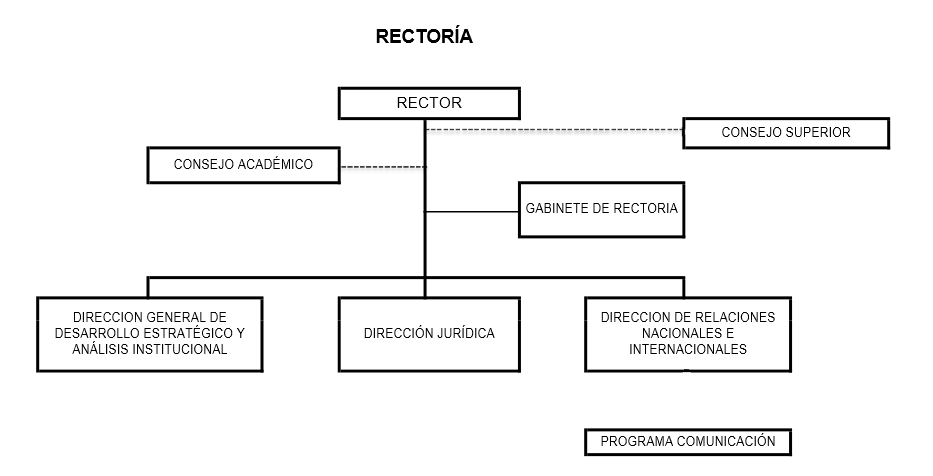
\includegraphics[scale=0.6,angle=0]{images/organigrama/1.png}
\caption{Organigrama de rector\'ia}
\label{Organigrama de rectoria}
\end{center}
\end{figure}

Es el segmento con mas poder en la organización universitaria, siendo este el foco central de las decisiones tomadas por los otros organismos. Es importante señalar que muchas de sus políticas provienen en gran medida de las necesidades y aspiraciones de las siguientes estructuras jerárquicas.

\subsection{Vicerrectoría Academica}
Es la entidad de que administra de manera local las decisiones de rectoría, hacia distintos polos como: Investigación, Dirección de evaluación, Dirección de docencia, Relaciones estudiantiles, Biblioteca, UTEM Virtual.
\begin{figure}[!hbp]
\begin{center}
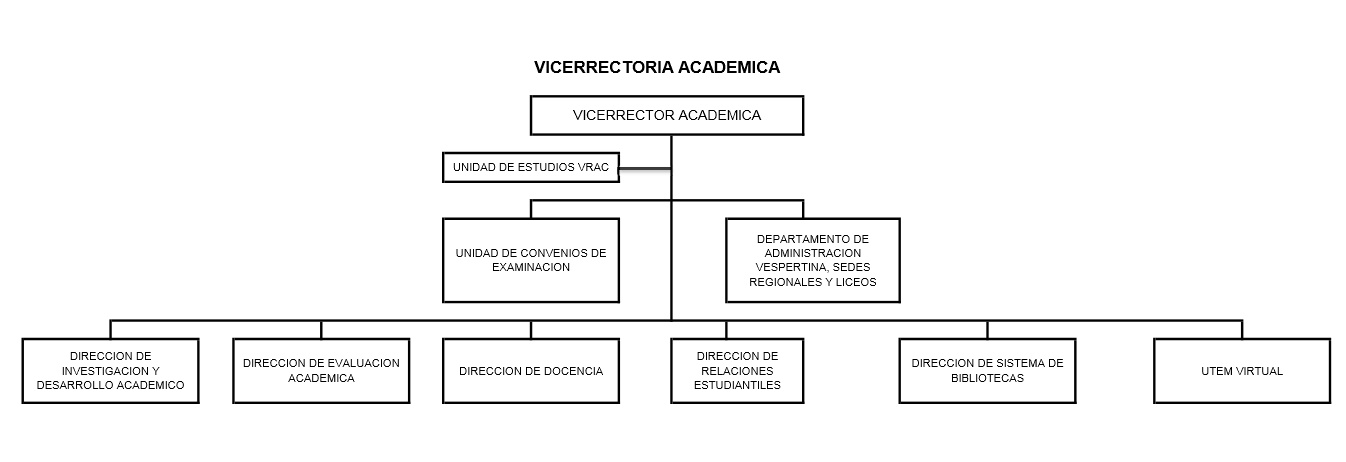
\includegraphics[scale=0.45,angle=0]{images/organigrama/2.png}
\caption{Organigrama de Vicerrector\'ia Academica}
\label{Organigrama de vicerrectoria Academica}
\end{center}
\end{figure}

Tiene el rol de velar por la correcta disponibilidad de recursos frente a los organismos de dirección institucional, para lo cual trabaja de manera constante en un perfeccionamiento de su rol como comandante.

\subsection{Facultad de ingeniería}
El decano de ingeniería es el principal responsable por las decisiones tomadas en esta estructura, debe liderar a todos los departamentos que le corresponden y cada uno de estos debe trabajar en pos de las directrices del decano de la facultad.
\begin{figure}[!hbp]
\begin{center}
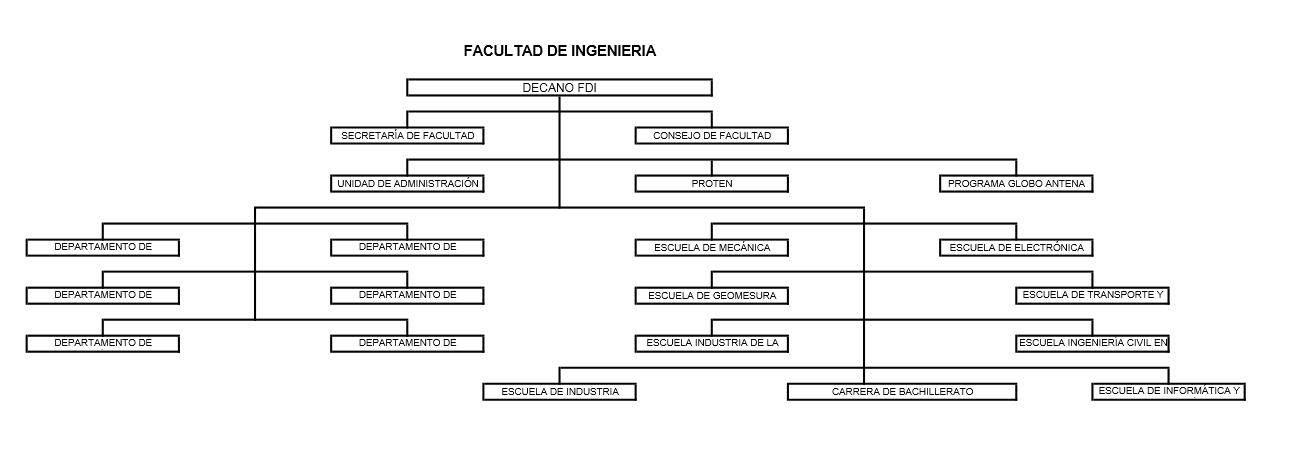
\includegraphics[scale=0.45,angle=0]{images/organigrama/11.png}
\caption{Organigrama de la facultad de ingen\'ieria}
\label{Organigrama de la facultad de ingenieria}
\end{center}
\end{figure}
\chapter{Anexo - PSP}
\thispagestyle{empty}
\section{Base teórica}
PSP (Proceso de Software Personal) es una metodología de desarrollo para proyectos informáticos, que tiene una serie de pasos enfocados en el ordenamiento, cuantificación y la categorización del trabajo y el tiempo. Es usada mundialmente por su fácil aprendizaje y su rápida incorporación. Este modelo de trabajo es solo para proyectos personales, o sea, en donde el desarrollador toma todo el trabajo por sí solo.

Este tipo de trabajo nos proporciona una serie de tablas que muestran nuestros tiempos de desarrollo y avance del proyecto, básicamente en el PSP nosotros podemos obtener los tiempos de desarrollo y la cantidad de líneas de código para cada actividad o conjunto de actividades. De esta manera uno puede llegar a determinar un factor de calidad dentro de nuestro trabajo dentro de los estándares que uno estime conveniente utilizar.

PSP nos obliga a desarrollar una forma de trabajo en la cual un desarrollador programa y anota los tiempos de desarrollo y la cantidad de código que uno ha producido, dentro de distintas tablas hechas para ese propósito.

\section{Ventajas y Desventajas}
Las ventajas del uso de PSP, básicamente están en el orden que genera, debido a que, desarrollar una aplicación grande siempre es un desafío, pero cuando se trabaja de forma ordenada, se encapsulan de mejor manera los errores que se producen en el desarrollo. Mientras que la principal desventaja es el tiempo que lleva, el aprender su metodología de trabajo, incorporarla al trabajo cotidiano y finalmente el resumen de los resultados. Esto produce que se gaste tiempo en actividades de calculo, en vez de ocuparlo en el desarrollo.

\section{Criterios para uso de PSP}
La necesidad de usar PSP fue concebida para generar un proyecto que tuviera un criterio de calidad cuantificable, ya que nos proporcionaba tablas e indicadores que establecen con el tiempo empleado, la cantidad de esfuerzo y errores que se pueden cometer en el trascurso del proyecto.

Se mostrará la forma de desarrollo de las tablas PSP más importantes en el proyecto dando cuenta de cómo es el desempeño del PSP dentro de nuestro proyecto SEPA. Tendremos el desarrollo de las tablas más importantes en el PSP frente a nuestra operación. Obtendremos una mirada clara respecto a que es el PSP y como éste permite complementar calidad en nuestra ocupación.

\section{Desarrollo del PSP}
\subsection{El trabajo del ingeniero de sofware}
En este apartado se listan las actividades que contempla el desarrollo del proyecto, incluyendo todo lo que pueda servir como avances. Para estos efectos se desarrollo la siguiente tabla de actividades, con su frecuencia horaria.

\newpage
\begin{table}
\begin{tabular}{|l | l | l |}
\hline
\textbf{Tarea} & \textbf{Frecuencia (semanal)} & \textbf{Tiempo (minutos)} \\
\hline
Estudiar documentos & todos & 840/semana\\
\hline
Desarrollo & todos & 1260\\
\hline
Programar & todos & 2520\\
\hline
Reuniones & L, M, J & 420/semana\\
\hline
Reparar Documentos & Mi, V & 840/semana\\
\hline
\end{tabular}
\caption{Tabla de actividades}
\end{table}
\subsection{La gestión del tiempo}
Para este punto solo se necesita la estructuración del tiempo que uno tiene sobre el tiempo que se pretende dar al proyecto, basándose en la lista de actividades. Se tienen todos los días de la semana destinados para el propósito de desarrollar el proyecto ya sea en informes o programar. En menos tiempo se reparten las tareas de investigar y reparar cosas.
\subsection{El control del tiempo}
Para este apartado se desarrolla una tabla que contiene una lista de actividades con los tiempos de inicio y término de cada una de las tareas que se hacen. También se anotan los tiempos perdidos, el tipo de actividad y si está completada o no. Se muestra la siguiente tabla de control de Tiempo, de forma resumida, para un día en especifico.
\newpage
\begin{table}
\begin{tabbing}
Estudiante: \= Miguel Angel Fuenzaldia Pino \= Fecha: \= 9/10/2012\\
Profesor: \> Sebastián Salazar Molina \>   \>  \\
\end{tabbing}
\begin{tabular}{| l | l | l | l | l | l | l | l | l |}
\hline
\textbf{Fecha} & \textbf{Comienzo} & \textbf{Fin} & \textbf{Delta} & \textbf{Actividad} & \textbf{Comentarios}\\
\hline
19/11 & 10:56 & 11:17 & 20 & Desarrollo & notebook\\
\hline
      & 11:18 & 11:35 & 15 & lectura & psp\\
\hline
      & 11:35 & 12:29 & 50 & Desarrollo & notebook\\
\hline
      & 12:30 & 12:56 & 30 & lectura & psp\\
\hline
      & 12:57 & 13:02 & 5 & Desarrollo & notebook\\
\hline
      & 13:02 & 13:29 & 30 & Almorzar & olgura\\
\hline
      & 13:30 & 15:21 & 120 & Desarrollo & notebook\\
\hline
      & 15:22 & 16:12 & 45 & lectura & psp\\
\hline
      & 15:22 & 16:00 & 40 & Desarrollo & notebook\\
\hline   
20/11 & 16:00 & 17:00 & 60 & Desarrollo & notebook\\
\hline
      & 17:00 & 18:26 & 90 & lectura & psp\\
\hline
      & 18:30 & 19:00 & 30 & Desarrollo & notebook\\
\hline 
21/11 & 18:00 & 18:30 & 30 & lectura & psp\\
\hline
      & 18:30 & 19:00 & 30 & Desarrollo & notebook\\
\hline 
26/11 & 15:00 & ... & ... & Desarrollo & notebook\\
\hline
\end{tabular}
\caption{Tabla de control de tiempo}
\end{table}
\subsection{Planificación de períodos y productos}
Este apartado se preocupa de la planificación semanal del tiempo, en la parte de desarrollo se tienen 3 tablas que nos permiten llevar los registros totales de tiempo en minutos de las actividades hecha durante la semana. La primera tabla muestra las sumas de los tiempos, la segunda muestra la actividad de las semanas pasadas y la tercera muestra el total de las semanas hasta hoy en día. Se muestran las siguientes tablas de planificación, de forma resumida, para comprender como se utilizan.

\begin{table}
\textbf{Estudiante}: Miguel Angel Fuenzaldia Pino     \textbf{Fecha}: 9/10/2012\\
\begin{tabular}{| l | l | l | l | l | l |}
\hline
\textbf{Tarea} & \textbf{Reunion} & \textbf{Codificar} & \textbf{Escribir} & \textbf{Leer} & \textbf{Total} \\
\hline
\textbf{Fecha} &                  & \textbf{Programas} & \textbf{Textos} & \textbf{textos} & \\
\hline
D 18/11 & & & & & \\
\hline
L & & 180 & 60 & 60 & 350\\
\hline
M & & & & & \\
\hline
Mi & & 180 & 60 & 60 & 350\\
\hline
J & 120 & & & & 120\\
\hline
V & & 180 & 60 & 60 & 350\\
\hline
S & & & & & \\
\hline
\textbf{Totales} & 120 & 540 & 180 & 180 & 1170\\
\hline
\end{tabular}
\caption{Primera tabla de planificación de periodos y productos}
\end{table}

Tiempos y Medias del Período, Número de Semanas (número anterior +1): 1\\
Resumen de las semanas anteriores:
\begin{table}
\begin{tabular}{| l | l | l | l | l | l |}
\hline
\textbf{Total} & 1170 & 1290 & 1170 & 1150 & 1170 \\
\hline
\textbf{Med.} & 1000 & 900 & 500 & 1000 & 1000 \\
\hline
\textbf{Máx} & 1170 & 1290 & 1170 & 1150 & 1170 \\
\hline
\textbf{Mín} & 900 & 800 & 400 & 900 & 800 \\
\hline
\end{tabular}
\caption{Segunda tabla de planificación de periodos y productos}
\end{table}

Resumen de las semanas totales (anteriores mas última)
\begin{table}
\begin{tabular}{| l | l | l | l | l | l |}
\hline
\textbf{Total} & 1170 & 2460 & 3630 & 4780 & 5950 \\
\hline
\textbf{Med.} & 1000 & 1900 & 2400 & 3400 & 4400 \\
\hline
\textbf{Máx} & 1170 & 2460 & 3630 & 4780 & 5950 \\
\hline
\textbf{Mín} & 900 & 1700 & 2100 & 3000 & 3800 \\
\hline
\end{tabular}
\caption{Tercera tabla de planificación de periodos y productos}
\end{table}
\subsection{La planificación del producto}
El desarrollo del proyecto requiere de un cuaderno que registre la actividad en función de los trabajos que se van realizando, para lo cual se tiene un cuaderno de trabajos que registra las actividades con sus respectivas estimaciones de tiempo, sacadas de datos anteriores. Recordar que en esta tabla se anotan los trabajos que resumen las actividades diarias, así que se anota uno al día. La siguiente tabla muestra una forma de planificación.
\newpage
\begin{table}
\textbf{Estudiante}: Miguel Angel Fuenzaldia Pino     \textbf{Fecha}: 9/10/2012\\
\begin{tabular}{|c|c|c|c|c|c|c|c|c|c|c|c|c|}
\hline
\textbf{Trab} & \textbf{Fecha} & \textbf{Pro} & \multicolumn{2}{|c|}{\textbf{Estimado}} & \multicolumn{3}{|c|}{\textbf{Real}} & \multicolumn{5}{|c|}{\textbf{Hasta la Fecha}} \\
\hline
 & & & \textbf{Tie} & \textbf{Uni} & \textbf{Tie} & \textbf{Uni} & \textbf{Vel} & \textbf{Tie} & \textbf{Uni} & \textbf{Vel} & \textbf{Máx} & \textbf{Mín} \\
\hline
\multirow{2}{*}{1} & 19/11 & Escr. & 420 & 1 & 300 & 2 & 150 & 300 & 2 & 150 & 150 & 150 \\
\cline{2-13} & \multicolumn{12}{|l|}{\textbf{Descripción:} Escribir el Engineer Notebook para los capitulos 5 al 12}\\
\hline
\multirow{2}{*}{2} & 20/11 & Escr. & 420 & 1 & 300 & 2 & 150 & 300 & 2 & 150 & 150 & 150 \\
\cline{2-13} & \multicolumn{12}{|l|}{\textbf{Descripción:} Escribir el Engineer Notebook para los capitulos 7 al 16}\\
\hline
\multirow{2}{*}{n} & & & & & & & & & & & & \\
\cline{2-13} & \multicolumn{12}{|l|}{\textbf{Descripción:}}\\
\hline
\end{tabular}
\caption{Tabla de la planificación de producto}
\end{table}
\subsection{El tamaño del producto}
Para estimar los costes de tiempo y valor de cada actividad que representa parte del desarrollo del un producto como tal, es necesario establecer formas de medición para valores que pueden ser cuantificables en unidades de trabajo. Para lo cual se mostrarán Estimaciones de Tamaños para las actividades particulares de este proyecto. Se tiene una muestra de tablas para determinar la cantidad total de trabajo que se realiza..
\newpage
\begin{table}
\begin{tabbing}
\textbf{Estudiante:} \= Miguel Angel Fuenzaldia Pino \= \textbf{Fecha:} \= 19/11/2012\\
\textbf{Profesor:} \> Sebastián Salazar Molina \> \textbf{Tiempos de Actividad} \>  \\
\end{tabbing}
\textbf{Reunión}\\
\begin{tabular}{| l | l | l | l |}
\hline
\textbf{Persona} & \textbf{Tiempo} & \textbf{Temas} & \textbf{Tiempo x Tema}\\
\hline
Sebastián Salazar & 60 & 4 & 15\\
\hline
\textbf{Totales} & 60 & 4 & 15 \\
\hline
\textbf{Medias} & 60 & 4 & 15 \\
\hline
\end{tabular}
\caption{Tabla del tamaño del producto}
\end{table}
\begin{table}
\textbf{Lectura}\\
\begin{tabular}{| l | l | l | l |}
\hline
\textbf{Capítulo} & \textbf{Tiempo} & \textbf{Páginas} & \textbf{Tiempo x Página}\\
\hline
1-5   & 180 & 50 & 3,6 \\
\hline
6-10  & & & \\
\hline
11-15 & & & \\
\hline
16-20 & & & \\
\hline
\textbf{Totales} & 180 & 50 & 3,6 \\
\hline
\textbf{Medias} & 180 & 50 & 3,6 \\
\hline
\end{tabular}
\caption{Tabla asociada a la lectura}
\end{table}
\begin{table}
\textbf{Escribir}\\
\begin{tabular}{| l | l | l | l |}
\hline
\textbf{Documento} & \textbf{Tiempo} & \textbf{Páginas} & \textbf{Tiempo x Página}\\
\hline
PSP & 360 & 30 & 20 \\
\hline
Bitácora & 10 & 1 & 10 \\
\hline
título & & & \\
\hline
\textbf{Totales} & 370 & 31 & 30 \\
\hline
\textbf{Medias} & 185 & 15,5 & 15 \\
\hline
\end{tabular}
\caption{Tabla asociada a escribir}
\end{table}
\begin{table}
\textbf{Programar}\\
\begin{tabular}{| l | l | l | l | l | l | l |}
\hline
\textbf{Programa} & \textbf{LOC} & \textbf{Func. Anteriores} & \textbf{Func. Hasta} & \textbf{Mín} & \textbf{Media} & \textbf{Máx}\\
\hline
Modelo & 			500  & 400 & 200 & 200 & 400 & 500 \\
\hline
Control &			100  & 50  & 25  & 25  & 50  & 100 \\
\hline
Vista &  			400  & 350 & 175 & 175 & 350 & 400\\
\hline
\textbf{Totales} &	1000 & 800 & 200 & 200 & 800 & 1000 \\
\hline
\textbf{Medias} & 	500	 & 400 & 100 & 100 & 400 & 500\\
\hline
\end{tabular}
\caption{Tabla asociada a programar}
\end{table}

\subsection{La gestión del tiempo}
Para poder desarrollar las actividades, se necesita tiempo, por lo cual resulta importante manejarlo apropiadamente, para esto se hace una estimación aproximada del tiempo que consumirá la ejecución de las actividades relacionadas con el desarrollo del trabajo que está en curso. Se expondrán dos tablas y un marco de referencias para las aproximaciones futuras. Se muestran las tablas de gestión del tiempo por actividades.
\begin{table}
\begin{tabbing}
\textbf{Estudiante:} \= Miguel Angel Fuenzaldia Pino \= \textbf{Fecha:} \= 19/11/2012\\
\textbf{Profesor:} \> Sebastián Salazar Molina \> \textbf{Tiempos de Actividad} \>  \\
\end{tabbing}
\textbf{Toma de Requerimientos y Preparación de Engineer Notebook}\\
\begin{tabular}{| l | l | l | l | l | l |}
\hline
\textbf{Tarea} & \textbf{Reunion} & \textbf{Codificar} & \textbf{Escribir} & \textbf{Leer} & \textbf{Total} \\
\hline
\textbf{Fecha} &                  & \textbf{Programas} & \textbf{Textos} & \textbf{textos} & \\
\hline
D  &    & & 180 & 180 & 360 \\
\hline
L  & 60 & & 180 & 180 & 420 \\
\hline
M  &    & & 180 & 180 & 360 \\
\hline
Mi & 60 & & 180 & 180 & 420 \\
\hline
J  &    & & 180 & 180 & 360 \\
\hline
V  & 60 & & 180 & 180 & 420 \\
\hline
S  &    & & 180 & 180 & 360 \\
\hline
\textbf{Totales} & 180 & & 1260 & 1260 & 1440 \\
\hline
\end{tabular}
\caption{Primera tabla de la gestión del tiempo}
\end{table}
\begin{table}
\textbf{Etapa de desarrollo de Proyecto e Informe}\\
\begin{tabular}{| l | l | l | l | l | l |}
\hline
\textbf{Tarea} & \textbf{Reunion} & \textbf{Codificar} & \textbf{Escribir} & \textbf{Leer} & \textbf{Total} \\
\hline
\textbf{Fecha} &                  & \textbf{Programas} & \textbf{Textos} & \textbf{textos} & \\
\hline
D  &    & 180 & 180 &  & 360 \\
\hline
L  & 60 & 180 & 180 &  & 420 \\
\hline
M  &    & 180 & 180 &  & 360 \\
\hline
Mi & 60 & 180 & 180 &  & 420 \\
\hline
J  &    & 180 & 180 &  & 360 \\
\hline
V  & 60 & 180 & 180 &  & 420 \\
\hline
S  &    & 180 & 180 &  & 360 \\
\hline
\textbf{Totales} & 180 & 1260 & 1260 &  & 2700 \\
\hline
\end{tabular}
\caption{Segunda tabla de la gestión del tiempo}
\end{table}
\subsection{La gestión de los compromisos}
Los compromisos que uno hace con las personas a las cuales espera entregar un proyecto, deben ser documentados, mostrando el tipo de actividad a realizar, el día, los participantes de ese compromiso, la hora en que se realiza, la fecha y finalmente lo que se recibe a cambio de la finalización de estas tareas. Es importante destacar que una correcta forma de manejar los compromisos lleva a un buen plan de trabajo. La siguiente tabla muestra un ejemplo de los compromisos y la información de acuerdo a cada tarea que uno pretende realizar.
\begin{table}
\begin{tabbing}
\textbf{Estudiante:} \= Miguel Angel Fuenzaldia Pino \= \textbf{Fecha:} \= 19/11/2012\\
\textbf{Profesor:} \> Sebastián Salazar Molina \> \textbf{Tiempos de Actividad} \>  \\
\end{tabbing}
\textbf{Lista de Compromisos}\\
\begin{tabular}{| l | l | l | l | l | l |}
\hline
\textbf{Fecha} & \textbf{Compromizo} & \textbf{¿Con quíen?} & \textbf{Horas} & \textbf{Fin} & \textbf{Consigo} \\
\hline
D  & Leer       & Propio   & 3 & Dom & Conocimiento \\
\hline
L  & Desarrollo & Cliente  & 3 & ... & título \\
\hline
M  & Escribir   & Profesor & 3 & ... & título \\
\hline
Mi & Desarrollo & Cliente  & 3 & ... & título \\
\hline
J  & Reunión    & Profesor & 1 & ... & Información \\
\hline
V  & Desarrollo & Cliente  & 3 & ... & título \\
\hline
S  & Escribir   & Profesor & 3 & ... & título \\
\hline
\end{tabular}
\caption{Tabla de la gestión de los compromisos}
\end{table}
\subsection{La gestión de las programaciones}
En un proyecto siempre es necesario definir las características importantes que comprenden la ejecución de cada una de las actividades que se están desarrollando, por tanto en este proyecto se tiene un registro de los puntos de control, los cuales representan las características importantes que el desarrollo de este trabajo debe comprender. A continuación una tabla que muestra un poco como una persona que utiliza el PSP puede programar su lista de actividades.
\begin{table}
\textbf{Estudiante}: Miguel Angel Fuenzaldia Pino     \textbf{Fecha}: 9/10/2012\\\\\
\begin{tabular}{| l | l |}
\hline
\multicolumn{2}{|c|}{\textbf{Puntos de Control}}\\
\hline
\textbf{Numero} & \textbf{Punto de Control}\\
\hline
1 & Desarrollar el Cuaderno de Anotaciones para la Metodología PSP \\
\hline
2 & Asistir a reuniones con el profesor encargado del ramo \\
\hline
3 & Desarrollar el Sofware que se pide, a traves de los requerimientos conseguidos \\
\hline
4 & Escribir un informe de título en coordinación con lo requerido\\
\hline
\end{tabular}
\caption{Tabla de la gestión de las programaciones}
\end{table}
\subsection{El plan del proyecto}
Para generar un plan del proyecto se necesita tener un resumen de las características de cómo se desarrolla el trabajo, para lo cual se expondrá un molde para generar planes de proyectos, mediante el cual se estima la cantidad de esfuerzo que uno puede desarrollar de acuerdo a las labores anteriores que ha realizado. Finalmente se mostrará un ejemplo de estimación del tamaño del programa. Se tiene un molde de lo que es el plan del proyecto, que es la parte más consistente del desarrollo en PSP, ya que nos muestra información acerca de tiempos por líneas de código en un compendio de actividades que puede ser una tarea a realizar semanalmente o en periodos más largos.
\begin{table}
\textbf{Resumen del plan de Proyecto}\\
\begin{tabular}{| l | l | l | l |}
\hline
\textbf{Estudiante:} & Miguel Angel Fuenzaldia Pino & \textbf{Fecha:} & 19/11/2012\\
\hline
\textbf{Programa:} & Sistema mantenedor e Integrador & \textbf{Programa No.:} & 5\\
\hline
\textbf{Profesor:} & Sebastián Salazar Molina & \textbf{Lenguaje} & Java  \\
\hline
\end{tabular}
\caption{Primera tabla del plan de proyecto}
\end{table}
\begin{table}
\begin{tabular}{| l | l | l | l | l | l |}
\hline
\textbf{Resumen} & \textbf{Plan} & \multicolumn{2}{|c|}{\textbf{Real}} & \multicolumn{2}{|c|}{\textbf{Hasta la Fecha}} \\
\hline
\textit{Minutos/LOC} & 0.5 & \multicolumn{2}{|c|}{\textbf{1}} & \multicolumn{2}{|c|}{\textbf{180}} \\
\hline
\textit{LOC/Hora} & 120 & \multicolumn{2}{|c|}{\textbf{40}} & \multicolumn{2}{|c|}{\textbf{250}} \\
\hline
\textit{Defectos/KLOC} & 4 & \multicolumn{2}{|c|}{\textbf{10}} & \multicolumn{2}{|c|}{\textbf{50}} \\
\hline
\textit{Rendimiento} & 0.5 & \multicolumn{2}{|c|}{\textbf{0.4}} & \multicolumn{2}{|c|}{\textbf{0.45}} \\
\hline
\textit{VIF} & 2 & \multicolumn{2}{|c|}{\textbf{}} & \multicolumn{2}{|c|}{\textbf{}} \\
\hline
\textbf{Tamaño(LOC)} & \multicolumn{5}{|c|}{\textbf{2500}}\\
\hline
\textit{Nuevo y Cambiado} & 500 & \multicolumn{2}{|c|}{\textbf{300}} & \multicolumn{2}{|c|}{\textbf{1000}} \\
\hline
\textit{Máx} & 1000 & \multicolumn{4}{|c|}{\textbf{}}\\
\hline
\textit{Mín} & 500  & \multicolumn{4}{|c|}{\textbf{}}\\
\hline
\textbf{Fase(Mín)} & \textbf{Plan} & \textbf{Real} & \textbf{Hasta la Fecha} & \multicolumn{2}{|c|}{\textbf{Porcentaje}} \\
\hline
\textit{Planificación} & 60 & 50  & 500  & \multicolumn{2}{|c|}{\textbf{0.16}}\\
\hline
\textit{Diseño} &        50 & 60  & 400  & \multicolumn{2}{|c|}{\textbf{0.19}}\\
\hline
\textit{Codificación} &  30 & 20  & 1000 & \multicolumn{2}{|c|}{\textbf{0.06}}\\
\hline
\textit{Revisión} &      20 & 60  & 500  & \multicolumn{2}{|c|}{\textbf{0.19}}\\
\hline
\textit{Compilación} &   50 & 20  & 100  & \multicolumn{2}{|c|}{\textbf{0.06}}\\
\hline
\textit{Pruebas} &       60 & 60  & 200  & \multicolumn{2}{|c|}{\textbf{0.19}}\\
\hline
\textit{Postmortem} &    50 & 40  & 200  & \multicolumn{2}{|c|}{\textbf{0.12}}\\
\hline
\textit{Total} &		320 & 310 & 3000 & \multicolumn{2}{|c|}{\textbf{1}}\\
\hline
\textit{Máx} & 			400	& \multicolumn{4}{|c|}{\textbf{}}\\
\hline
\textit{Mín} & 			200 & \multicolumn{4}{|c|}{\textbf{}}\\
\hline
\end{tabular}
\caption{Segunda tabla del plan de proyecto}
\end{table}
\newpage
\begin{table}
\begin{tabular}{| l | l | l | l | l | l |}
\hline
\textbf{D. Introducidos} & \textbf{Plan} & \textbf{Real} & \textbf{Hasta la Fecha} & \textbf{Porcentaje} & \textbf{Def./Hora} \\
\hline
\textit{Planificación} &  6 & 12 & 60 & 0.16 & 2\\
\hline
\textit{Diseño} &		  8 & 16 & 80 & 0.22 & 2\\
\hline
\textit{Codificación} &  10 & 20 &100 & 0.27 & 4\\
\hline
\textit{Revisión} &       5 & 10 & 50 & 0.14 & 1\\
\hline
\textit{Compilación} &    4 &  8 & 40 & 0.11 & 1\\
\hline
\textit{Pruebas} &        3 &  6 & 30 & 0.08 & 1\\
\hline
\textit{Total} &         36 & 74 & 360& 1 & 11 \\
\hline
\textbf{D. Eliminados} & \textbf{Plan} & \textbf{Real} & \textbf{Hasta la Fecha} & \textbf{Porcentaje} & \textbf{Def./Hora} \\
\hline
\textit{Planificación} &  6 & 12 & 60 & 0.16 & 2\\
\hline
\textit{Diseño} &		  8 & 16 & 80 & 0.22 & 2\\
\hline
\textit{Codificación} &  10 & 20 &100 & 0.27 & 4\\
\hline
\textit{Revisión} &       5 & 10 & 50 & 0.14 & 1\\
\hline
\textit{Compilación} &    4 &  8 & 40 & 0.11 & 1\\
\hline
\textit{Pruebas} &        3 &  6 & 30 & 0.08 & 1\\
\hline
\textit{Total} &         36 & 74 & 360& 1 & 11 \\
\hline
\end{tabular}
\caption{Tercera tabla del plan de proyecto}
\end{table}
\subsection{Defectos}
El registro de los defectos es altamente importante, ya que nos permite la correcta verificación de cada incidente ocurrido dentro del proceso de desarrollo del software. El cuaderno de registro de errores se ocupa en el proceso de desarrollo de aplicaciones, y nos permite anotar un error cuando ha salido en modo de compilación para lo cual uno registra el tipo de error y el tiempo dedicado a la reparación de este error. El objetivo de esta tabla es impedir la repetición de ciertos errores que pueden ser reparados mediante el aprendizaje.\\
\begin{table}
\textbf{Tipos de Defectos}\\
\begin{tabular}{| l | l | l | l |}
\hline
10 & Documentación         & 60 & Comprobación\\
\hline
20 & Sintaxis              & 70 & Datos\\
\hline
30 & Construcción Paquetes & 80 & Función\\
\hline
40 & Asignación            & 90 & Sistema\\
\hline
50 & Interfaz              & 100 & Entorno\\
\hline
\end{tabular}
\caption{Primera tabla defectos}
\end{table}

La siguiente tabla es simplemente una muestra de la lista de los defectos y como se van anotando.
\begin{table}
\textbf{Resumen del plan de Proyecto al cual se le encuentran Defectos}\\
\begin{tabular}{| l | l | l | l |}
\hline
\textbf{Estudiante:} & Miguel Angel Fuenzaldia Pino & \textbf{Fecha:} & 19/11/2012\\
\hline
\textbf{Programa:} & Sistema mantenedor e Integrador & \textbf{Programa No.:} & 5\\
\hline
\textbf{Profesor:} & Sebastián Salazar Molina & \textbf{Lenguaje} & Java  \\
\hline
\end{tabular}
\caption{Segunda tabla defectos}
\end{table}
\begin{table}
\begin{tabular}{| l | l | l | l | l | l | l |}
\hline
\textbf{Fecha} & \textbf{Número} & \textbf{Tipo} & \textbf{Introducido} & \textbf{Eliminado} & \textbf{Correc.} & \textbf{Correg.}\\
\hline
2013-07-13 & 30 & 1 & 2013-07-13 & 2013-07-18 & si & no \\
\hline
\textbf{Descripción} & \multicolumn{6}{|c|}{Mal despliegue de textos, en mantenedores} \\
\hline
\end{tabular}
\caption{Tercera tabla defectos}
\end{table}


\end{document}
